\chapter{processes}
\label{ch:processes}
\pagestyle{fancy}

\fancyhf{} % here we clear any fancy header settings
%% Note, the first page of every chapter does not have a header.
\fancyhead[EC]{Linux System Administration} % E = even pages, C = center, rightmark defaults to number of current section
\fancyhead[OC]{\leftmark} % O=odd pages, C= center, leftmark defaults to Chapter number and title

%%
%% Set, headheight to eliminate warning message "Package Fancyhdr Warning: \headheight is too small (12.0pt): Make it at least 13.59999pt.
\setlength{\headheight}{13.6pt} 
%%
% The next line would put a line at the bottom of every page starting from the second page of every chapter, if it was uncommented.
%%
%\renewcommand{\footrulewidth}{1pt}
%%
\cfoot{\thepage} % c = center, foot = footer, thepage = page number
\rhead{
\includegraphics[width=.5cm]{figures/smCanadianFlag}}
		
%%%%%%%%%%%%%%%%%%%%%%%%%%%%%%%%%%%%%%%%%%%%%%%%%%%%%%%%%%%
%%%%%%%%%%%%%%%%%%%%%%%%%%%%%%%%%%%%%%%%%%%%%%%%%%%%%%%%%%%
\section{Introduction}
 As with any operating system, Linux runs some applications as background processes. These processes are either started automatically when the system starts or when they are manually started by a logged on user. So, we need some way of interacting with these background processes. Fortunately, Linux comes with an abundance of command line tools that help us see how these processes interact with the system (CPU and memory consumption). As well, the tools allow one to configure and manage the processes in real time.
 
 \section{ps}
 
 The \keyword{ps} command is used to get a snapshot of the current running processes. The amount of information displayed about a selection of the active processes depends on the ps options or switches used and the filters applied...usually with \keyword{grep} or \keyword{awk}.
 
 \subsection{processes by terminal}
 
 \begin{itemize}
 	\item \tbi{PID: }All processes have a process ID or PID that the Linux kernel uses to uniquely identify an active process.
 	\item \tbi{TTY: }The name of the terminal connected to standard input.
 	\item \tbi{TIME: }The cumulative CPU time used by the active process since inception.
 	\item \tbi{CMD: }The executable name of the process.
 \end{itemize}
 
\begin{lstlisting}[escapeinside={¿}{¿},frame=single,breaklines,columns=fixed]
 #
 # What's my psuedo terminal id?
 #
 ¿\tld¿ tty
 /dev/pts/1
 #
 # ps by itself tells us little. We see that we are running bash in psuedo terminal slave 1:  pts/1. Each terminal window has a unique tty with names in this format: pts/number.
 #
 ¿\tld¿ ps
 PID   TTY      TIME     CMD
 11875 pts/1    00:00:00 ps
 31589 pts/1    00:00:00 bash 
 
 ¿\tld¿ ps t
 PID   TTY      TIME     CMD
 11875 pts/1    00:00:00 ps
 31589 pts/1    00:00:00 bash 
 #
 # In the above, we used the t or terminal option. When no argument is given, ps returns the process information for the current terminal. Let's get the process information for another terminal window.
 #
 ¿\tld¿ ps t pts/3
 PID  TTY      STAT   TIME COMMAND
 3217 pts/3    Ss+    0:00 /bin/bash	
 \end{lstlisting}

\section{Time for a snooze}
 
Now, let's run the \keyword{sleep} and \keyword{echo} commands in the background so that we can regain control of the terminal session. If we do not put the ampersand at the end of the statement, the terminal would be locked until the \emph{sleep} and \emph{echo} commands finished processing.

\begin{itemize}
  	\item \tbi{sleep }Delay for 300 seconds (1 minute), don't do anything.
  	\item \tbi{; }A command separator.
  	\item \tbi{echo "meme" > ./sleepy }Echo or send the string "meme" to the file \textsl{sleepy} in the current directory. This happens after the 300 second sleep.
  	\item \tbi{\& }Run both processes in the background, note the use of the brackets. Without the brackets, only the second command would run in the background. Putting an ampersand after each command would also not work.
\end{itemize}  

\begin{lstlisting}[escapeinside={¿}{¿},frame=single,breaklines,columns=fixed]
¿\tld¿ ( sleep 300 ; echo "meme" > ./sleepy) &
[1] 17267

# Immediately after issuing the above command, we issue the ps command again. We see that bash is used to start the sleep command. No mention is given of the second command, echo. Why? echo will run only after the sleep command finishes. It would be very difficult to time the issue of the ps command to capture the execution of this echo command.
#
¿\tld¿ ps
PID   TTY      TIME     CMD
17267 pts/1    00:00:00 bash
17269 pts/1    00:00:00 sleep
17280 pts/1    00:00:00 ps
31589 pts/1    00:00:00 bash
#
# After one minute, issue the ps command again.
#
¿\tld¿ ps
PID TTY        TIME     CMD
17722 pts/1    00:00:00 ps
31589 pts/1    00:00:00 bash
[1]+  Done                    ( sleep 60; echo "meme" > ./sleepy )
#
# Did the echo command run? Yes, as can be seen by displaying the contents of the file: sleepy. We can also infer that this write took place by reading the last output line from the above ps command.
#
¿\tld¿ cat sleepy
meme
\end{lstlisting}

So, how do the two commands work in conjunction with each other? We can conclude from the following output that the \emph{echo} command is executed only after the first command has finished. Note, in the command below, I changed the \emph{sleep} value to 10 seconds and appended the output of the \emph{echo} command to the file \textsl{sleepy}...using the double greater-than symbol >{}>{}. If I had used a single >, the file would have been overwritten.

\begin{lstlisting}[escapeinside={¿}{¿},frame=single,breaklines,columns=fixed] 
¿\tld¿ ( sleep 10 ; echo "meme" >> ./sleepy) &
[1] 5177
#
# Let's get the process list.
#
¿\tld¿ ps
PID  TTY      TIME     CMD
5177 pts/1    00:00:00 bash
5179 pts/1    00:00:00 sleep
5187 pts/1    00:00:00 ps
31589 pts/1   00:00:00 bash
#
# After 10 seconds...
#
¿\tld¿ ps
PID   TTY       TIME     CMD
5222  pts/1     00:00:00 ps
31589 pts/1     00:00:00 bash
[1]+  Done                    ( sleep 10; echo "meme" >> ./sleepy )
#
# So, only one "meme" was appended to the file: sleepy...it already contained a ling with the string "meme".
#
¿\tld¿ cat sleepy
meme
meme
\end{lstlisting}

\section{psuedo terminal IDs and Terminator}\label{subsec:terminator}
 
In the above section, I mentioned that each terminal has its own psuedo terminal ID. I use the \tbi{Terminator} terminal emulator in a 2 row by 2 column configuration. Take a look at the following image. Each terminal window has a unique \tbi{pts/ID}.\\ 
 
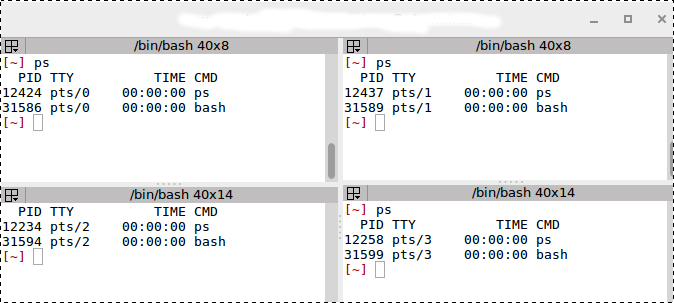
\includegraphics[width=1\textwidth]{figures/ps}\\
 
If you want this type of 2x2 layout, make a backup of \textsl{\ttb{}.config/terminator/config}. Next, recreate the \textsl{config} file with the following settings.\\
  
\begin{lstlisting}[escapeinside={¿}{¿},frame=single,breaklines]
  [global_config]
  enabled_plugins = CustomCommandsMenu, TestPlugin, TerminalShot, APTURLHandler, LaunchpadCodeURLHandler, LaunchpadBugURLHandler
  [keybindings]
  [layouts]
  [[default]]
  [[[child0]]]
  fullscreen = False
  last_active_term = c3520923-b680-4510-98c9-131e08a16f17
  last_active_window = True
  maximised = True
  order = 0
  parent = ""
  position = 0:27
  size = 1920, 986
  title = mgcr@LIB2015:~/.config/terminator
  type = Window
  [[[child1]]]
  order = 0
  parent = child0
  position = 958
  ratio = 0.500260416667
  type = HPaned
  [[[child2]]]
  order = 0
  parent = child1
  position = 489
  ratio = 0.498478701826
  type = VPaned
  [[[child5]]]
  order = 1
  parent = child1
  position = 489
  ratio = 0.498478701826
  type = VPaned
  [[[terminal3]]]
  order = 0
  parent = child2
  profile = default
  type = Terminal
  uuid = c3520923-b680-4510-98c9-131e08a16f17
  [[[terminal4]]]
  order = 1
  parent = child2
  profile = default
  type = Terminal
  uuid = c6dbb19a-0746-48ba-a9c5-576b6399243e
  [[[terminal6]]]
  order = 0
  parent = child5
  profile = default
  type = Terminal
  uuid = 6892246c-ee46-412a-82f9-ea15d0399865
  [[[terminal7]]]
  order = 1
  parent = child5
  profile = default
  type = Terminal
  uuid = 24723eb5-0621-4567-9305-ff7f8c3664c3
  # one is the old default			 
  [[one]]
  [[[child1]]]
  parent = window0
  type = Terminal
  [[[window0]]]
  parent = ""
  type = Window
  [plugins]
  [profiles]
  [[default]]
  background_image = None
  copy_on_selection = True
  scrollback_infinite = True	
  \end{lstlisting}
 
 For a quick look at other terminal emulators, please visit this URL: \href{https://opensource.com/life/15/11/top-open-source-terminal-emulators?sc\_cid=701600000011kF7AAI}{Top 7 open source terminal emulators}.

\subsection{controlling terminal IDs}

We can issue the command \tbi{stty -a} to find all the commands that help change and print terminal line settings. For example, we can see that \textasciicircum{}Z or CTRL+Z is used to suspend a running process in a termial window.\\

\begin{lstlisting}[escapeinside={¿}{¿},frame=single,breaklines]
¿\tld¿ stty -a
speed 38400 baud; rows 31; columns 117; line = 0; intr = ^C; quit = ^\; erase = ^?; kill = ^U; eof = ^D; eol = M-^?; eol2 = M-^?; swtch = M-^?; start = ^Q; stop = ^S; susp = ^Z; rprnt = ^R; werase = ^W; lnext = ^V; discard = ^O; min = 1; time = 0; -parenb -parodd -cmspar cs8 hupcl -cstopb cread -clocal -crtscts -ignbrk brkint -ignpar -parmrk -inpck -istrip -inlcr -igncr icrnl ixon -ixoff -iuclc ixany imaxbel iutf8 opost -olcuc -ocrnl onlcr -onocr -onlret -ofill -ofdel nl0 cr0 tab0 bs0 vt0 ff0 isig icanon iexten echo echoe echok -echonl -noflsh -xcase -tostop -echoprt echoctl echoke -extproc
\end{lstlisting}

\section {tty and pts}
For a quick discussion of \keyword{tty} and \keyword{pts}, read this URL: \href{http://unix.stackexchange.com/questions/93531/what-is-stored-in-dev-pts-files-and-can-we-open-them}{Stack Exchange}.

\begin{itemize}
\item \tbi{TTY} ports are usually direct connections to the computer such as a keyboard/mouse or a serial connection to the device. Old UNIX boxes would have dozens of of devices plugged into the back, all connected with cables. However, today system processes not initiated at a pseudo terminal slave are connected to a numbered tty: tty0, tty1, tty2

\item \tbi{PTS} stands for pseudo terminal slave. A terminal (or console) session needs one physical keyboard/screen combination that you sit and type at. However, from there you can create may pseudo terminal slave connections.  Remote SSH or telnet connections also initiate a pseudo terminal slave. Regardless, pseudo terminal slaves are numbered sequentially: pts/0, pts/1,...pts/n. In a way, pseudo terminal slaves are a virtual type of connection to the system.
\item \tbi{/DEV} Poke around in this folder and you will see that \keyword{tty} and \keyword{pts} files reside in this folder. \keyword{dev} is a special folder that contains device files for all devices. 
\end{itemize}

My observation is as follows:

\begin{enumerate}
	\item {Every process is connected to either a \emph{tty} or a \emph{pts}.} 
	\item {Processes connected to a \emph{tty} are started by the system or by a user from the desktop environment, i.e., launch the application using Gnome GUI menus.}
	\item {Processes connected to a \emph{pts} are started by a user at a terminal window, an ssh shell or simple bash terminal window.}
\end{enumerate}	

Ok, so let's list all of the processes running under the user \emph{mgcr}. Note that, in the code below, that I started the \keyword{ps} command at \emph{ps/0}, psuedo terminal slave 0, my first bash window. All other processes are connected to \emph{tty2}.  All other processes were either started by the system or started as a GUI application...such as \emph{texstudio} and \emph{chrome}.

\begin{lstlisting}[escapeinside={¿}{¿},frame=single,breaklines,columns=fixed,columns=fixed]	
¿\tld¿ ps -u mgcr | grep -E 'tty|pts'
5703   tty2     00:00:00 gvfsd-http
9535   tty2     00:00:36 texstudio
114271 tty2     00:00:00 evinced
21548  pts/0    00:00:00 ps
21549  pts/0    00:00:00 grep
.
.
24217  tty2     00:00:04 firefox
24569  tty2     00:11:12 opera:libflashp
24648  tty2     00:00:02 opera:libgnome-
#
# Note, when we pipe to grep, we loose our header. To get the header back, you can do the following. The first command up to the ';' prints the heading only. If you just issued the command 'ps -u mgcr', without the grep, you would also get the header information.
#
¿\tld¿ ps | head -1; ps -u mgcr | grep -E 'tty|pts'
   PID TTY      TIME     CMD
  5703 tty2     00:00:00 gvfsd-http
  9535 tty2     00:00:36 texstudio
114271 tty2     00:00:00 evinced
 21548 pts/0    00:00:00 ps
 21549 pts/0    00:00:00 grep
.
.
.
24217  tty2     00:00:04 firefox
24569  tty2     00:11:12 opera:libflashp
24648  tty2     00:00:02 opera:libgnome-
#
# So, we see that firefox is connected to tty2. I then closed firefox and started it (in the background with the command: firefox &)from the bash terminal . Note, it is now running as a pts/1 process where previously it ran at tty2.
#
¿\tld¿ firefox &
[1] 3571
¿\tld¿ ps -u mgcr | grep -E 'tty|pts' | grep firefox
3571 pts/1    00:00:05 firefox
#
# I closed firefox again, but this time I launched it from Gnome's Application Menu. Note, it is again running as a tty.
#
¿\tld¿ ps -u mgcr | grep -E 'tty|pts' | grep firefox
3849 tty2     00:00:05 firefox
\end{lstlisting}

\subsection{Be quiet, shh or is it ssh?}

Is it really that important to know to what type of terminal session a process is connected? Maybe and maybe not? For example, suppose I want to get a list of users who are remotely connected to my system using \keyword{ssh - secure shell}. In the example below, we see that one user is connected to our system using \emph{ssh} and that that connection is a psuedo terminal slave connection: \emph{pts/6}. What piece of information is more relevant, useful, or important? \tbi{Knowing} the terminal connection type? or \tbi{Knowing} who is connected and what type of connection protocol is being used?

\begin{lstlisting}[escapeinside={¿}{¿},frame=single,breaklines,columns=fixed]
#
# sshd is the secure shell daemon or process that permits users to remotely connect to a system using the ssh protocol.
#
# grep -v grep, just removes listing the grep command itself from the process list. Try the command without: grep -v grep.
#
# ps -aux, print a list of all user processes.
#	
¿\tld¿ ps -aux | grep -E 'tty|pts' | grep sshd | grep -v grep
mgc  6410  0.0  0.0 170796  4340 ?    S   08:52   0:00 sshd: mgc@pts/6
#
# Note: I grepped two things: terminal session type, tty or pts, and the sshd process. Let's remove the first grep that is grepping the termnal type.
#
¿\tld¿ ps -aux | grep sshd | grep -v grep
root 1558  0.0  0.0  81412  5772 ?    Ss   Jan17   0:00 /usr/sbin/sshd -D
root 6377  0.0  0.0 170796  9132 ?    Ss   08:52   0:00 sshd: mgd [priv]
mgc  6410  0.0  0.0 170796  4340 ?    S    08:52   0:00 sshd: mgd@pts/6
#
# So, we still get the sshd process connected to the pts, but we also get the main sshd process itself and a spawned sshd process started by user: mgc.
#
# grep is a very powerful tool that can help isolate information.  If you do not understand what you are doing, it can also easily hide information that may be relevant to your investigation.
#
# What if we wanted a bit more information about the remote connection?
#
# w = who is logged, what time did they connect, what are they doing?
#
# who = who is logged on, what date and time did they connect, and from where?
#
# w, tells us that user mgc started a pseudo teminal slave connection from a bash terminal, that started at 08:52, no other process has been started by: mgc.
#
# who, gives us similar information. User mgc started a pts connection, but in addition to time of day, we also get the date and more importantly the source IP address of the connection...which in this case is from another system on the local area network.
#
¿\tld¿ w | grep mgc
mgc      pts/6     08:52   32:12   0.02s  0.02s -bash

¿\tld¿ who | grep mgc
mgc      pts/6        2016-01-19 08:52 (192.168.0.18)
\end{lstlisting}

\begin{tabularx}{\linewidth}{>{\bfseries}X | X} % the X is needed to wrap text
\caption{Processes by Terminals}\label{table:processes-terminals}\\ % title of Table
\toprule
\normalfont{Command} & Action \\% inserts table heading, unbolds 1st column heading
\midrule
ps -ef grep -E \tqs{tty|pts} & full-format listing of all processes filtered on type of connection using grep's regex switch\\[2mm]
ps -ef grep \tqs{tty\textbackslash{}|pts} & full-format listing of all processes filtered on type of connection, regular grep with escape character before the \emph{logical or} symbol\\[2mm]
ps -ft pts/0 -t pts/2 -t tty1 & full-format listing of all processes on three terminals: pts/0, pts/2, and tty1\\[1mm]
ps -t pts/0 -t pts/2 -t tty1 & partial-format listing of all processes on three terminals: pts/0, pts/2, and tty1\\[1mm]
w & who is logged on and what are they doing,  a very condensed list, one per terminal\\[1mm]
who & who is logged on to terminals\\[1mm]
who am i & who am i (my user name) and on what terminal\\[1mm]
whoami & just show my user name\\[1mm]
\bottomrule
\end{tabularx}

\subsection{Horton the...}

Let's look at the \keyword{who} command in detail. Not only can we get information about users and terminal sessions, but we can also get information on the current run-level and the time and date of the last system boot.

\begin{lstlisting}[escapeinside={¿}{¿},frame=single,breaklines,columns=fixed]
#
# List the switches for the who command. Note, I am going to use the -H option often since I want to see the header.
#	
¿\tld¿ m- who # my .bashrc function 'm-'
-a, --all
-b, --boot
-d, --dead
-H, --heading 
-l, --login
--lookup
-m     only hostname and user associated with stdin
-p, --process
-q, --count
-r, --runlevel
-s, --short
-t, --time
-T, -w, --mesg
-u, --users
--message
--writable
--help display this help and exit
--version
#
# Let's start by getting just a list of logged on users, nothing else. The cut delimeter is a space. We want only the first field. We also want to sort this field and eliminate duplicates. We just want unique names. In this case '| uniq | sort' will also work. 
#
¿\color{red}{\textit{Be careful when using these two commands together: uniq and sort. If you don't get the result that you expect, try switching the order of the two commands.}}¿
#
¿\tld¿ who | cut -d' ' -f1 | sort | uniq
mgc
mgcr

#
# Who is logged on to terminal sessions? The options, -Hs and -T, would also produce the same output.
#
¿\tld¿ who -H
NAME LINE         TIME             COMMENT
mgcr tty2         2016-01-17 08:01 (:0)
mgcr pts/0        2016-01-17 08:01 (:0)
mgcr pts/1        2016-01-17 08:01 (:0)
mgcr pts/2        2016-01-17 08:01 (:0)
mgcr pts/3        2016-01-17 08:01 (:0)
mgc  pts/6        2016-01-19 08:52 (192.168.0.18)

#
# Get system boot time, runlevel, and terminal session info for all users.
#
¿\tld¿ who -Ha
NAME       LINE         TIME             IDLE          PID COMMENT  EXIT
           system boot  2016-01-17 19:54
           run-level 5  2016-01-17 19:55
           pts/0        2016-01-17 20:45              4524 id=ts/0  term=0 exit=0
mgcr + 	   tty2         2016-01-17 08:01  old        22295 (:0)
mgcr +     pts/0        2016-01-17 08:01 00:49       22797 (:0)
mgcr +     pts/1        2016-01-17 08:01 04:08       22797 (:0)
mgcr +     pts/2        2016-01-17 08:01   .         22797 (:0)
mgcr +     pts/3        2016-01-17 08:01 00:23       22797 (:0)
mgc      + pts/6        2016-01-19 08:52 04:51        6377 (172.18.0.18)
#
# Who is logged on at this terminal?
#
¿\tld¿ who -Hm
NAME     LINE         TIME             COMMENT
mgcr     pts/2        2016-01-17 08:01 (:0)
# 
# What is the run-level?
#
¿\tld¿ who -Hr
NAME     LINE         TIME             IDLE          PID COMMENT
         run-level 5  2016-01-17 19:55
#
# What users are logged on?
#
¿\tld¿ who -Hu
NAME LINE         TIME             IDLE          PID COMMENT
mgcr tty2         2016-01-17 08:01  old        22295 (:0)
mgcr pts/0        2016-01-17 08:01 00:04       22797 (:0)
mgcr pts/1        2016-01-17 08:01 04:18       22797 (:0)
mgcr pts/2        2016-01-17 08:01   .         22797 (:0)
mgcr pts/3        2016-01-17 08:01 00:32       22797 (:0)
mgc  pts/6        2016-01-19 08:52 05:01       6377 (192.168.0.18)

\end{lstlisting}

\subsection {Sending messages to users}
Ok, all well and nice, but how do we actually use all this information? A typical scenario is one where we need to reboot a server. Let's say we issued the \emph{who} command and saw that several users were connected. One by one, we could send a message to each user. In the following example, I am using my 2x2 terminal grid. I am going to send a message from my \emph{pts/0} terminal window to my \emph{pts/3} terminal window.

\begin{lstlisting}[escapeinside={¿}{¿},frame=single,breaklines]
#
# Sending from pts/0
#
¿\tld¿ who am i
mgcr pts/0        2016-01-17 08:01 (:0)
#
# After issuing the following command and hitting the enter key, you are taken to the next blank line. You then begin writing the message on consecutive lines or as one big line. Use CTRL+Z to end and send the message. Each time you hit the enter key, that line is sent to the other terminal.
#
¿\tld¿ write mgcr pts/3
hi there
system going down in 5 minutes...please close all applications and log off
^Z
[4]+  Stopped                 write mgcr pts/3
#
# An alternative to typing individual lines of the message followed CTRL+Z is to simply echo the information and pipe it to the write command.
#
¿\tld¿ echo "Hi, there! The system is going down in 5 minutes...time to panic!" | write mgcr pts/3
#
# What would I see on pts/3? I issue the 'who am i' command to show that I am on that terminal.
#
¿\tld¿ who am i
mgcr pts/3        2016-01-17 08:01 (:0)
#
# Then, immediatedly after I issue the write command on pts/0, this message appears...
#
¿\tld¿ 
Message from mgcr@LIB2015 on pts/0 at 14:05 ...
#
# And, as I type a line and hit the enter key, each line is displayed in succession. Unfortunately, at the destination prompt, there is no indication that more messages follow. The only way you know that there are no more messages is when you hit the enter key and are returned to the command prompt.
#
hi there
system going down in 5 minutes...please close all applications and log off
#
# Well, what if you had 100 users logged on? You certainly would not send 100 individual messages! You can instead use the wall command, which sends the same message to all users.
#
¿\tld¿ wall "system going down"

Broadcast message from mgcr@LIB2015 (pts/0) (Sun Jan 17 14:13:46 2016):  

system going down
#
# What would you see on each terminal window?
#
¿\tld¿
Broadcast message from mgcr@LIB2015 (pts/0) (Sun Jan 17 14:13:46 2016):  
system going down
#
# If you had a recurring event, you would want to send the same message each time. The best way to do this is to store your messages into files and then use standin to send the files to the wall command. Note, even the terminal session from which you send the message receives the message.
#
# The greater than symbol sends output or writes to the destination file: sgd.msg. The less than symbol sends the information the other direction. The contents of sgd.msg are sent to the wall command as input.
#
¿\tld¿ echo "system going down in 5 minutes...please close all applications and log off" > sgd.msg
¿\tld¿ wall < sgd.msg

Broadcast message from mgcr@LIB2015 (pts/0) (Sun Jan 17 14:27:27 2016):  

system going down in 5 minutes...please close all applications and log off   
#
# But, this just sends the message, it does not actually do anything about the reboot.
#
¿\tld¿ shutdown -r +15 "Server is going down in the middle of the day in order to create havoc and make you work less efficiently...all within the next 15 minutes. Please don't save ALL your work and do ignore this message!"  
#
# The above command schedules a system reboot in 15 minutes time and immediately sends out a message to all users logged onto the system.
#
\end{lstlisting}

In the above section, we used the \keyword{shutdown} command with its messaging feature. Please be aware that this method will not work for users at a different shell level than you and as well it will not send a message to users with a network connection such as: \tbi{ftp}, \tbi{smtp}, \tbi{pop3}, \tbi{tftp}, \tbi{ssh}. \textit{It is best to schedule shutdown and reboot times during a maintenance window that has been previously established and communicated to all users via email or some other messaging service.}

\section{Breaking a complex command into parts}

In the following table, I am just dabbling with the \keyword{w} command and showing how one can break a complex command into smaller steps. The web can be a great source of information and you will often find solutions to your problems or challenges. However, quite often the code in the solutions can be quit complex. \textit{I strongly recommend that you try to break the code down into its parts so that I understand each part.} I am going to illustrate this approach, but in reverse order. I start with a simple command and add more complex parts.

\begin{lstlisting}[escapeinside={¿}{¿},frame=single,breaklines,columns=fixed]
¿\tld¿ w
10:48:54 up 1 day, 14:54,  6 users,  load average: 3.69, 3.53, 3.39
USER TTY       LOGIN@  IDLE    JCPU   PCPU  WHAT
mgcr tty2      Mon08   38:54m  2days  0.04s opera:libflashp
mgcr pts/0     Mon08    2.00s  0.16s  0.00s w
mgcr pts/1     Mon08    1:13m  0.10s  0.10s /bin/bash
mgcr pts/2     Mon08    2:48m  0.06s  0.06s /bin/bash
mgcr pts/3     Mon08   10:54   0.14s  0.14s /bin/bash
mgc  pts/6     08:52    1:56m  0.02s  0.02s -bash
#
# Interesting...it looks like there are only 6 processes running, five for user mgcr on one for user mgc.
#
# Also, there is only one process on tty2. Is that correct? Let's use the ps command to list processes and filter on terminal tty2. We will also get a count of those processes on tty2.
# The first part of the command list our processes: ps -ft tty2
# The command separator is the semi-colon.
# The second part of the command pipes its output to 'wc -l', count the number of lines, the result is: 81.
#
# We use the ps command with the -f (full-format) and -t (terminal type) switches to get a list of only processes running on tty2.
#
¿\tld¿ ps -ft tty2 ; ps -ft tty2 | wc -l
UID   PID  PPID  C STIME TTY   TIME       CMD
mgcr  2146    1  0 Jan18 tty2  00:00:24   javaws.itweb -splash:/usr/share/icedtea-web/javaws_splash.png -Xbootc
mgcr  2212 2146 99 Jan18 tty2  1-09:26:52 javaws.itweb -splash:/usr/share/icedtea-web/javaws_splash.png -Xboo
.
.
mgcr 29929 22805 3 11:09 tty2  00:00:00   [opera:libflashp] <defunct>
81
¿\tld¿
#
# So, removing the line count for the heading, mgcr has 80 processes running on tty2. I elided most of the process listing which is indicated by the two vertical periods.
#
# Ok, what we eventually want to do is to loop through each terminal type in order to see the running processes for each terminal type. We begin by using the output of the w command to get a simple list of all terminal types, which is listed in column 2 of the output of this command. We use awk to isolate column 2, represented by {print $2}.
#
¿\tld¿ w | awk '{print $2}'
up
TTY
tty2
pts/0
pts/1
pts/2
pts/3
pts/6
# 
# We need to get rid of the first two rows. Why? Drop the pipe to see full output of w. As above, we only want the second column. We use 'grep -v', inverse grep, to remove the two lines. That is the lines containing: up or TTY. Another option to remove the two lines would be to use the sed command. ¿\textbf{\color{red}Challenge:} How would you do that? \hyperlink{sedel}{Answer.}¿
#
¿\tld¿ w | awk '{print $2}' | grep -v "up\|TTY"
tty2
pts/0
pts/1
pts/2
pts/3
pts/6
#
# Alright, now let's loop through all these terminals.
#
¿\tld¿ for trm in `w | awk '{print $2}' | grep -v "up\|TTY"`; do ps -ft $trm;done
¿\textbf{\color{red}UID        PID  PPID  C STIME TTY          TIME CMD}¿
mgcr 2146     1  0 Jan18 tty2  00:00:25  javaws.itweb -splash:/usr/share/icedtea-web/javaws_splash.png -Xbootc
mgcr 2212  2146 99 Jan18 tty2  -10:07:16 javaws.itweb -splash:/usr/share/icedtea-web/javaws_splash.png -Xboo
.
.
mgcr 32307 31952  0 11:21 tty2     00:00:00 /opt/google/chrome/chrome --type=renderer --lang=en-GB --force-fieldt
¿\textbf{\color{red}UID        PID  PPID  C STIME TTY          TIME CMD}¿
mgcr  2592 23027  0 11:34 pts/0    00:00:00 ps -ft pts/0
mgcr 23027 22797  0 Jan18 pts/0    00:00:00 /bin/bash
¿\textbf{\color{red}UID        PID  PPID  C STIME TTY          TIME CMD}¿
mgcr 23030 22797  0 Jan18 pts/1    00:00:00 /bin/bash
¿\textbf{\color{red}UID        PID  PPID  C STIME TTY          TIME CMD}¿
mgcr 23035 22797  0 Jan18 pts/2    00:00:00 /bin/bash
¿\textbf{\color{red}UID        PID  PPID  C STIME TTY          TIME CMD}¿
mgcr 23040 22797  0 Jan18 pts/3    00:00:00 /bin/bash
¿\textbf{\color{red}UID        PID  PPID  C STIME TTY          TIME CMD}¿
mgc       6421  6410  0 08:52 pts/6    00:00:00 -bash
#
# Ugh, note, it prints the heading at the beginning of each terminal type...let's remove the heading using the --no-heading switch for ps.
#
¿\tld¿ for trm in `w | awk '{print $2}' | grep -v "up\|TTY"`; do ps --no-heading -ft $trm;done
mgcr  2146     1  0 Jan18 tty2     00:00:25 javaws.itweb -splash:/usr/share/icedtea-web/javaws_splash.png -Xbootc
mgcr  2212  2146 99 Jan18 tty2     1-10:11:26 javaws.itweb -splash:/usr/share/icedtea-web/javaws_splash.png -Xboo
.
.
mgcr 32307 31952  0 11:21 tty2     00:00:00 /opt/google/chrome/chrome --type=renderer --lang=en-GB --force-fieldt
mgcr  2968 23027  0 11:36 pts/0    00:00:00 ps --no-heading -ft pts/0
mgcr 23027 22797  0 Jan18 pts/0    00:00:00 /bin/bash
mgcr 23030 22797  0 Jan18 pts/1    00:00:00 /bin/bash
mgcr 23035 22797  0 Jan18 pts/2    00:00:00 /bin/bash
mgcr 23040 22797  0 Jan18 pts/3    00:00:00 /bin/bash
mgc   6421  6410  0 08:52 pts/6    00:00:00 -bash
#
# As an aside, I noticed that mgcr and mgd did not have any processes on tty1.  Who does? It turns out that only the user with UID gdm, the GNOME Display Manager, has processes on that terminal.
#
¿\tld¿ ps -ft tty1
UID  PID  PPID  C STIME TTY      TIME     CMD
gdm  1671 1609  0 Jan17 tty1     00:00:00 /usr/libexec/gdm-wayland-session /usr/bin/gnome-session --autostart /
.
.
.
gdm       2072  1943  0 Jan17 tty1     00:00:00 /usr/libexec/ibus-engine-simple
\end{lstlisting}

So, typically you may find a complex command on the Internet such as this command...

\begin{lstlisting}[escapeinside={¿}{¿},frame=single,breaklines,columns=fixed]
for trm in `w | awk '{print $2}' | grep -v "up\|TTY"`; do ps --no-heading -ft $trm;done
\end{lstlisting}

Your task would be to break down this command into its smaller parts, the reverse of what I did in building up to my final command. This is a tremendous way of learning! \textit{Don't just find and use commands without fully understanding  what they do.} You will quickly advance your learning and skill set if you dissect complex commands you find on the Internet.

\subsection{How to get just one header}

Ok, what if we wanted only that initial heading? Here is some code that will print the heading once and only once. It uses a counter called \emph{count} and a \emph{for} loop. The header is printed on the first iteration through the loop when count=1. Save this file as \textsl{pts.sh} and then \emph{chmod u+x pts.sh} to make it executable. To run the code, type: \emph{bash pts.sh} or \emph{./pts.sh}. You will get a list of all processes sorted by terminal type with the heading only at the beginning of the output.

\begin{lstlisting}[escapeinside={¿}{¿},frame=single,breaklines]
¿\tbi{\#}¿/bin/bash
# Print heading only on first iteration through the loop.
count=0
for trm in `w | awk '{print $2}' | grep -v "up\|TTY"`
do
#
# Note: the counter statement uses (( ... )) but the 'if' statement uses [[ ... ]]. Also, pay attention to the spaces inside the curved and square brackets.
#
(( count++ ))    
if [[ $count -eq 1 ]]
then
ps -ft $trm
else
ps --no-heading -ft $trm
fi
done
\end{lstlisting}

\section{User processes}

Let's return to the \keyword{sleep} command. I am logged on as user \emph{mgcr}. When I issue just the \keyword{ps} command, I am only getting the processes for the pseudo terminal session. What about the processes for \emph{mgcr}?

\begin{lstlisting}[escapeinside={¿}{¿},frame=single,breaklines,columns=fixed]
¿\tld¿ (sleep 60 ; echo "meme" > ./sleepy) &
[1] 19967

¿\tld¿ ps
PID   TTY      TIME     CMD
14821 pts/1    00:00:00 bash
19967 pts/1    00:00:00 bash
19969 pts/1    00:00:00 sleep
19977 pts/1    00:00:00 ps
#
# Is the sleep process one of mine?
#
¿\tld¿ ps -u mgcr | grep sleep
19969 pts/1    00:00:00 sleep
#
# After 60 seconds, let's grep for "echo"...we could have also grepped for "sleep".
#
¿\tld¿ ps -u mgcr | grep echo
[1]+  Done                    ( sleep 60; echo "meme" > ./sleepy )	
\end{lstlisting}

\subsection{User processes - splitting hairs}
As above, we can get a list of all processes for a specific user. In the code below, I issue the \emph{ps -u mgcr} command to get a list of all processes started by the user \emph{mgcr}. In the following examples, I give only a snippet of the process list. As you can see, mgcr appears that we have 113 processes running. But, do we really?

\begin{lstlisting}[escapeinside={¿}{¿},frame=single,breaklines,columns=fixed]
¿\tld¿ whoami
mgcr
	
¿\tld¿ ps -u mgcr
PID  TTY      TIME     CMD
2176 ?        00:00:00 systemd
2177 ?        00:00:00 (sd-pam)
.
.
28392 tty2    00:00:13 evince
28399 tty2    00:00:00 evinced
#
# wc -l = print the newline counts
#
¿\tld¿ ps -u mgcr | wc -l
113
#
# But, this is rather cumbersome...we are using two commands; one to get a list of the processes and another to get a count of the running processes.
#
# Alternatively, we can pipe our output to bash's nl command in order to prepend the line number of each line. Note: piping to 'cat -n' will give the same result.
#
# We have to subtract one from the result because our count includes the heading. So, it looks like mgcr has 113 processes running, not 114.
#
¿\tld¿ ps -u mgcr | nl
1 PID     TTY      TIME     CMD
2 2176    ?        00:00:00 systemd
3 2177    ?        00:00:00 (sd-pam)
.
.
113 28392 tty2     00:00:13 evince
114 28399 tty2     00:00:00 evinced
#
# Let's try stripping the heading from our list. Below, I illustrate three ways of doing this. Only use one of these methods at a time.
#
¿\tld¿ ps -u mgcr | awk '{if(NR>1)print}' | nl
¿\tld¿ ps -u mgcr | sed -n '1!p' | nl
¿\tld¿ ps -u mgcr | tail -n +2 | nl
#
# All three of these commands produce the following listing...
#
1 2176    ?        00:00:00 systemd
2 2177    ?        00:00:00 (sd-pam)
.
.
113 28392 tty2     00:00:13 evince
114 28399 tty2     00:00:00 evinced
#
# Why is the count not 113?
#
# Answer: Each solution pipes to an additional command: awk, or sed, or tail. So, we are adding one additional process and removing the heading...which balances out. Just remember that when you issue a pipe, you are adding a process. 
#
# So, is the number of running processes 113?
#
# The number of running processes is actually 110! ¿\textbf{\color{red}Say, what?}¿
#
# To get our actual count of the total number of running processes, we have to remove the count for the heading, the count for 'wc -l' itself, and the count for 'ps -u mgcr'.
#
# Interesting or totally irrelevant? Hmmm...
#
\end{lstlisting}

\subsection{Counting user processes - the Harley metric}

There is an easy way to find out the number of user processes for each user on a system. These metrics may be helpful if your system is bogging down and you want a quick check to find the \tbi{hog} of all your system resources. I present the command and then create an alias called \emph{hog}. Trust me, you will often use this alias.

\begin{lstlisting}[escapeinside={¿}{¿},frame=single,breaklines]
#
# Note: 'sort' before 'uniq'...go ahead and try it the other way! Only two columns of information are generated: total user processes and user name.
#
¿\tld¿ ps -eo user=|sort|uniq -c
2 avahi
1 chrony
1 colord
1 dbus
25 gdm
1 lp
4 mgd
126 mgcr
1 nobody
1 polkitd
1 qemu
173 root
1 rtkit
#
# Hmm, the above command sorted by user name. Let's sort by descending order of the count.  -n=numeric, -r=reverse
#
¿\tld¿ ps -eo user=|sort|uniq -c | sort -n -r
174 root
127 mgcr
25 gdm
4 mgd
2 avahi
1 rtkit
1 qemu
1 polkitd
1 nobody
1 lp
1 dbus
1 colord
1 chrony
#
# You expect me to remember that command? Ok, let's create a command alias and add it to our .bashrc file. Pay attention to the different types of quotations that are used! We then just call the function by typing hog...after we have sourced .bashrc.
#
¿\tld¿ echo "alias hog='ps -eo user=|sort|uniq -c | sort -n -r'">>~/.bashrc

¿\tld¿ tail -1 ~/.bashrc
alias hog='ps -eo user=|sort|uniq -c | sort -n -r'

¿\tld¿ hog
174 root
127 mgcr
25 gdm
4 mgd
2 avahi
1 rtkit
1 qemu
1 polkitd
1 nobody
1 lp
1 dbus
1 colord
1 chrony

\end{lstlisting}

\section{Filtering process information}

\subsection{Introduction}

The simple \keyword{ps} command provides a ton of information. You will definitely want to read the manpage for \emph{ps} as there are many command switches and options that help to isolate and filter the information.

\subsection{ps switches/options explained} 

For the next discussion of \keyword{ps}, I want to use some specific switches that allow us to see all running processes.

\begin{itemize}
	\item[] \tbi{-A }Select all processes. Identical to -e.
	\item[] \tbi{-e }Select all processes. Identical to -A. 
	\item[] \tbi{-a }All processes except both session leaders (see getsid(2)) and processes not associated
	\item[] \tbi{-f }  Do full-format listing.
	\item[] \tbi{-o } Format, i.e., options, what to print.  
\end{itemize}

\subsection{examples of ps switch/options - filtering process fields}

\begin{lstlisting}[escapeinside={¿}{¿},frame=single,breaklines,columns=fixed]
#
# If you recall from the start of this chapter, the ps command by itself just presents process info for the bash terminal window.
#
¿\tld¿ ps
PID   TTY      TIME     CMD
7770  pts/3    00:00:00 ps
23040 pts/3    00:00:00 bash
#
# Let's get a count of all running processes.
#
¿\tld¿ ps aux | wc -l
333
#
# We can also use the -ef switch. Note, there is a small difference in the count.
#
¿\tld¿ ps -ef | wc -l
336
#
# We can also use the -Af switch.
#
¿\tld¿ ps -Af | wc -l
336
#
# Suppose I wanted a count of just the process containing the string "gdm"?
#
¿\tld¿ ps -ef | grep gdm | wc -l
31
#
# Ok, let's just list the 1st four of those processes.
#
¿\tld¿ ps -ef | head -4 | grep gdm
¿\tld¿ 
#
# Hmm, nothing was returned. Why? The order of the piping was incorrect. I asked to filter the first full lines of the output. But, in that output, no line contained "gdm". Therefore, the second pipe 'grep gdm' returned nothing. Switch the order. Put the head statement after the grep statement.
#
¿\tld¿ ps -ef | grep gdm | head -4
root  1579     1  0 Jan17 ?     00:00:00 /usr/sbin/gdm
root  1609  1579  0 Jan17 ?     00:00:00 gdm-session-worker [pam/gdm-launch-environment]
gdm   1630     1  0 Jan17 ?     00:00:00 /usr/lib/systemd/systemd --user
gdm   1632  1630  0 Jan17 ?     00:00:00 (sd-pam)
#
# Note two things from the above output. The string "gdm" was under both the UID and CMD column headers. How do I know these column headers?
#
¿\tld¿ ps -ef | head -1
UID        PID  PPID  C STIME TTY          TIME CMD
#
# So, how do I get the column header as well as the process information? And, just display the UID and CMD columns? I am going to use the awk's 'Output Field Separator=OFS' switch with the OFS equal to a tab, \t. To get the UID and CMD headers only, I know that I need to print only columns 1 and 8. 
#
¿\tld¿ ps -ef | head -1 | awk -v OFS='\t' '{print $1,  $8}'
UID		CMD
#
# Ok, that prints the heading. We just need to add the command to grep "gdm" and display only the first 4 lines of process information.
#
¿\tld¿ ps -ef | head -1 | awk -v OFS='\t' '{print $1,  $8}' ; ps -ef | grep gdm | head -4 | awk -v OFS='\t' '{print $1, $8}'
UID¿\qquad¿CMD
root¿\qquad¿/usr/sbin/gdm
root¿\qquad¿gdm-session-worker
gdm¿\qquad¿/usr/lib/systemd/systemd
gdm¿\qquad¿(sd-pam)
#
# Pretty cool! Is this command another candidate for a function?
#
# Here are some variations on awk formatting. In the first command, I am putting a fixed 5 spaces between the double-quotations. In the second command,I am using \t for one tab...which by default equals 5 spaces.
#
¿\tld¿ ps -ef | head -1 | awk '{print $1 "     " $8}'
UID¿\qquad¿CMD

¿\tld¿ ps -ef | head -1 | awk '{print $1 "\t" $8}'
UID¿\qquad¿CMD
#
# We can also get the same information with the 'ps aux' command. Here, I want the 1st and 11th column headers and the first 4 processes in the process list.
#
¿\tld¿ ps aux | awk '{print $1, $11}' | head -4
USER COMMAND
root /usr/lib/systemd/systemd
root [kthreadd]
root [ksoftirqd/0]
#
# And, of course, as soon as we grep, we loose our heading.
#
¿\tld¿ ps aux | awk '{print $1, $11}' | grep gdm | head -4
root /usr/sbin/gdm
root gdm-session-worker
gdm /usr/lib/systemd/systemd
gdm (sd-pam)
#
# Let's tet the heading back.
#
¿\tld¿ ps aux | awk '{print $1, $11}' | head -1 ; ps aux | awk '{print $1, $11}' | grep gdm | head -4
USER COMMAND
root /usr/sbin/gdm
root gdm-session-worker
gdm /usr/lib/systemd/systemd
gdm (sd-pam)
#
# Let's format the output a little differently...using tabs and pipe to less so that we can page through the screens of information. Hit the q key to quit the less pager.
#
¿\tld¿ ps aux | awk '{print $1, "\t", $2, "\t", $10, "\t", $11}' | less
USER     PID     TIME    COMMAND
root     1       0:02    /usr/lib/systemd/systemd
root     2       0:00    [kthreadd]
.
.
root     31      0:00    [kworker/3:0H]
root     32      0:05    [rcuos/3]
:
#
# Come on, there must be an easier way, awk seems so cumbersome?
#
# How about just printing four of the gdm processes and only output the pid and cmd fields? Really, can we call the fields by name?
#
¿\tld¿ ps -eo pid,cmd | grep gdm | head -4
1579 /usr/sbin/gdm
1609 gdm-session-worker [pam/gdm-launch-environment]
1671 /usr/libexec/gdm-wayland-session /usr/bin/gnome-session --autostart /usr/share/gdm/greeter/autostart  --session gnome-wayland
1705 /usr/libexec/gnome-session-binary --autostart /usr/share/gdm/greeter/autostart --session gnome-wayland
#
# It gets really tricky once you start playing with ps options.
#
¿\tld¿ ps -ef | head -2
UID        PID  PPID  C STIME TTY TIME     CMD
root         1     0  0 Jan17 ?   00:00:28 /usr/lib/systemd/systemd --switched-root --system --deserialize 21
#
# Alright, let's just get the UID and PID columns
#
¿\tld¿ ps -eo uid,pid | head -2
UID   PID
0     1
#
# Ok, no problem there, the output is consistent.
#
¿\tld¿ ps -efo uid,pid | head -2
UID        PID
1858215107 22295
#
# Just a sec, I simply added the full-format switch and now my UID is 1858215107.
#
¿\tld¿ id -u root
0
¿\tld¿ id -u mgcr
1858215107
# 
# So, with just the -eo switch, the first processes listed are for root whose UID is 0. With -efo, the first processes listed are for mgcr, the user that is logged on. Note: this value is the EUID system variable, the effective user ID.
#
¿\tld¿ ps -efo uid,pid  | grep gdm | head -2
¿\tld¿
#
# Hey, nothing was returned...after digging a little deeper in the man page...
#
¿\tld¿ ps -eo ruser=RealUser -o pid  | grep gdm | head -2
gdm       1630
gdm       1632
#
# Awesome, how about the header?
#
¿\tld¿ ps -eo uid,pid | head -1; ps -eo ruser=RealUser -o pid  | grep gdm | head -2
UID   PID
gdm   1630
gdm   1632
¿\tld¿ 
\end{lstlisting}

\subsection{AIX Format Descriptors (and making an alias out of a function)}

The \keyword{AIX FORMAT DESCRIPTORS} section of the \keyword{ps} manpage provides useful information about headers that we can use in our \emph{ps} commands. Until you can remember all these descriptors, you will want a quick way to display them. We can display the descriptors using my \emph{.bashrc mang} function. However, even this would be cumbersome to type each time you wanted to display the descriptors. How about creating an alias from a specific use of the \emph{mang} function. As the manpage describes, we can use any of the following descriptors: \emph{code, normal, header}.


\begin{lstlisting}[escapeinside={¿}{¿},frame=single,breaklines,columns=fixed]
#
# Here is my 'mang' function...
#
¿\tld¿ grep -A12 "function mang" .bashrc
function mang()
#
# This is another way of printing a section of a manpage.
# Change section headers to uppercase using echo and tr.
# Use the A (after) and B (before) grep switches with large values that ensure we just capture the section.
# $1 = manpage $2 = first header and $3 = second header
# Example: mang sed name synopsis
# 
{
b=`echo $2 | tr '[a-z]' '[A-Z]'`
e=`echo $3 | tr '[a-z]' '[A-Z]'`
man $1 | col -b| grep -A1000 -x "$b" | grep -B1000 -x "$e" | sed '$d'
}
#
# So, let's use my mang function to print the aix format descriptors section of the ps manpage
#
¿\tld¿ mang ps "aix format descriptors" "standard format specifiers"
AIX FORMAT DESCRIPTORS
This ps supports AIX format descriptors, which work somewhat like the formatting codes of printf(1) and  printf(3).  For example, the normal default output can be produced with this: ps -eo "%p %y %x %c".  The NORMAL codes are described in the next section.

CODE   NORMAL   HEADER
%C     pcpu     %CPU
%G     group    GROUP
%P     ppid     PPID
%U     user     USER
%a     args     COMMAND
%c     comm     COMMAND
%g     rgroup   RGROUP
%n     nice     NI
%p     pid      PID
%r     pgid     PGID
%t     etime    ELAPSED
%u     ruser    RUSER
%x     time     TIME
%y     tty      TTY
%z     vsz      VSZ
¿\tld¿
#
# Ok, let's create an alias out of this specific mang function and append it to the end of my .bashrc file. We are going to create an alias called: aix.
#	
¿\tld¿ echo "alias aix='mang ps "aix format descriptors" "standard format specifiers"'" >>.bashrc
#
# I can issue the 'source .bashrc' command to re-read my .bashrc file.
#
¿\tld¿ source .bashrc

¿\tld¿ aix
AIX FORMAT DESCRIPTORS
This ps supports AIX format descriptors, which work somewhat like the formatting codes of printf(1) and printf(3).  For example, the normal default output can be produced with this: ps -eo "%p %y %x %c".  The NORMAL codes are described in the next section.

CODE   NORMAL   HEADER
%C     pcpu     %CPU
%G     group    GROUP
%P     ppid     PPID
%U     user     USER
%a     args     COMMAND
%c     comm     COMMAND
%g     rgroup   RGROUP
%n     nice     NI
%p     pid      PID
%r     pgid     PGID
%t     etime    ELAPSED
%u     ruser    RUSER
%x     time     TIME
%y     tty      TTY
%z     vsz      VSZ
\end{lstlisting}

Ok, le's start using the different \keyword{aix} descriptors in our \keyword{ps} commands. Obviously, we only need our \keyword{aix} function to call up our table whenever we want to see the full \keyword{AIX FORMAT DESCRIPTORS} list.

\begin{lstlisting}[escapeinside={¿}{¿},frame=single,breaklines,columns=fixed]
#
¿\tld¿ ps -eo "%U %p %C" | head -3
USER 	PID %CPU
root 	1    0.0
root 	2    0.0
#
# There is an alternative to the above command where we drop the parentheses. There is no space between each code descriptor. If you put a space without the double-quotations, you would get an error message. Notice that 'head -3' includes the header as one component of the list.
#
¿\tld¿ ps -eo %U%p%C | head -3
USER       PID %CPU
root         1  0.0
root         2  0.0
#
# Using the normal descriptors.
#
¿\tld¿ ps -eo user,pid,pcpu | head -3
USER       PID %CPU
root         1  0.0
root         2  0.0
#
# Ok, let's do some sorting. We are going to display the ruser, pid, and nice values. Note, only when we sort on column 2 do we get the header.
# sort options: -n = numeric sort, -nr = reverse numeric sort, -k = sort to column
#
¿\tld¿ ps -eo %u%p%n | sort -n -k 2 | head -6
RUSER      PID  NI
root         1   0
root         2   0
root         3   0
root         4   0
root         5 -20
#
# Let's sort on column 1, the real user name.
#
¿\tld¿ ps -eo %u%p%n | sort -n -k 1 | head -6
avahi      945   0
avahi      959   0
chrony     924   0
colord    1593   0
dbus       917   0
gdm       1632   0
#
# Let's sort on column 3, the nice value.
#
¿\tld¿ ps -eo %u%p%n | sort -n -k 3 | head -6
root       101 -20
root       103 -20
root       108 -20
root       110 -20
root       111 -20
root       144 -20
#
# Let's do a reverse sort on column 3, largest to smallest nice value.
#
¿\tld¿ ps -eo %u%p%n | sort -nr -k 3 | head -6
root       904  19
root        39  19
mgcr 	  2855  19
mgcr      2820  19
root        38   5
rtkit      908   1
#
# A bit of cheese and whine..but, I want the headers...
#
¿\tld¿ ps -eo %u%p%n | head -1 ; ps -eo %u%p%n | sort -nr -k 3 | head -6
RUSER      PID  NI
root       905  19
root        39  19
mgcr      2813  19
mgcr      2800  19
root        38   5
rtkit      906   1
#
# Hey, hey, did you see that? I got all top 6 processes that I requested not header plus 5 processes. Do I focus on detail? Maybe! Have I asked that question before? Maybe!
#
\end{lstlisting}

\section{Finding top consumers of computer resources}\label{sec:topcpu}

At the most inconvenient of times, servers will start to bog down as they run out of computing resources. We already covered how to find users who are running the most number of processes. We can also do a search to find the top processes that are consuming CPU and Memory resources.

\begin{lstlisting}[escapeinside={¿}{¿},frame=single,breaklines,columns=fixed]
#
# Let's sort by descending order of memory usage.
#
¿\tld¿ ps -eo pid,uname,cmd,pmem,pcpu --sort=-pmem | head -5
PID   USER  CMD                         %MEM %CPU
12745 qemu  /usr/bin/qemu-system-x86_64 26.1 12.4
3849  mgcr  /usr/lib64/firefox/firefox   3.3  2.3
2212  mgcr  javaws.itweb -splash:/usr/s  2.9  160
22805 mgcr  /usr/lib64/opera/opera       2.2 19.5
#
# Let's now sort by descending CPU usage.
#
¿\tld¿ ps -eo pid,uname,cmd,pmem,pcpu --sort=-pcpu | head -5
PID   USER  CMD                         %MEM %CPU
2212  mgcr  javaws.itweb -splash:/usr/s  2.9  160
22307 mgcr  /usr/libexec/Xorg vt2 -disp  1.1 61.4
16255 mgcr  /opt/google/chrome/chrome -  1.1 26.1
22805 mgcr  /usr/lib64/opera/opera       2.2 19.5
#
# Ok, let's use a slightly different approach...this comand was issued a bit later so the process data is slightly different.
#
¿\tld¿ ps axo pid,args,pmem,rss,vsz --sort -pmem,-rss,-vsz | head -n 5
PID  COMMAND                     %MEM    RSS     VSZ
2951 /usr/lib64/firefox/firefox   2.5 623112 2491152
2828 /usr/lib64/opera/opera       2.0 492420 1356268
2615 /usr/bin/gnome-shell         1.5 372808 2391872
3524 /opt/google/chrome/chrome -  1.5 370540 1370892
#
# Suppose we want a real-time monitor running in one of our bash windows that would update every 10 seconds. To do this we use the watch command.
#
¿\tld¿ watch -n 10 'ps -eo pid,uname,cmd,pmem,pcpu --sort=-pcpu | head -5'
Every 10.0s: ps -eo pid,uname,cmd,pmem,pcpu --sort=-pcpu | head -5                           Thu Jan 21 08:47:32 2016

PID  USER  CMD                         %MEM %CPU
2782 mgcr  /usr/lib64/opera/opera       1.8 14.0
4680 mgcr  /usr/lib64/opera/pluginwrap  0.5  3.2
2565 mgcr  /usr/bin/gnome-shell         1.5  3.0
2878 mgcr  /usr/lib64/firefox/firefox   1.2  2.6
#
# This information would refresh every 10 seconds. CTRL+C to end.
#
\end{lstlisting}

\section{pids}

\subsection{Introduction}

Every process or application that is started is assigned a unique \emph{process id} or \emph{pid}. 

\subsection{Working with PIDs}

\begin{lstlisting}[escapeinside={¿}{¿},frame=single,breaklines,columns=fixed]
#
# Display the last 10 processes in our process list.
#
~] ps aux | tail -10
mgcr 14803  0.3  0.1 962800 37116 tty2     Sl+  08:46   0:00 /usr/bin/gedit
root 14818  0.0  0.0      0     0 ?        S    08:46   0:00 [kworker/1:3]
.
.
mgcr 15930  0.0  0.0 112208  1804 pts/2    S+   08:50   0:00 tail -10
#
# Let's just display the full-format PID information for two of these processes by specifying their PIDs.
#
¿\tld¿ ps -fp 14803,14818
UID   PID    PPID  C STIME TTY    TIME     CMD
mgcr  14803     1  0 08:46 tty2   00:00:00 /usr/bin/gedit
root  14818     2  0 08:46 ?      00:00:00 [kworker/1:3]
#
# Each running process has a directory in the /proc directory. Inside this process directory, there are a large number of files related to the process.
#
¿\tld¿ man proc | grep -x DESCRIPTION -A3
DESCRIPTION
The  proc  filesystem  is a pseudo-filesystem which provides an interface to kernel data structures.  It is commonly mounted at /proc.  Most of it is read-only, but some files allow kernel variables to be changed.
# 
# Ok, let's take a peek at the files for the process with PID 14803. Let's do a long-listing first.
#
¿\tld¿ ls -la /proc | grep 14803
dr-xr-xr-x.   9 me mygrp               0 Jan 21 08:46 14803
#
# How many files/folders? As you can see this PID has 728 files associated with it...some within subfolders of the 14803 directory.
#
¿\tld¿ find /proc/14803 -type f | wc -l
728
#
# We can get limited information about a process using just the ps command followed by a process ID.
#
¿\tld¿ ps 32503
PID 	TTY      STAT   TIME COMMAND
32503 	?        S      0:00 [kworker/0:3]
#
# However, if we add the u option, more information is provided.
#
¿\tld¿ ps u 32503
USER       PID %CPU %MEM    VSZ   RSS TTY   STAT START   TIME COMMAND
root     32503  0.0  0.0      0     0 ?     S    14:04   0:00 [kworker/0:3]
\end{lstlisting}	

\section{Killing Processes}

\subsection{Introduction}

So, what happens when we have a runaway process that is out of control and eating up available CPU and memory resources? We have to end or kill that process.

\subsection{Using \emph{yes} and \emph{sleep} to test running processes}

In the following examples, I am going to make use of the \keyword{yes} command. If you type this command at the console, an endless stream of \emph{y's} will appear at the console. The \emph{yes} command may not make a lot of sense, but it is commonly used if you need to pipe the \emph{yes} string "y" to another command in order to answer positively yes to a series of questions...such as during installation of a program.

I am also going to start the \emph{yes} program in the \emph{background} and redirect the standard output of \emph{yes} to \textsl{/dev/null}. Any data sent to \textsl{/dev/null} disappears, it acts as a black hole.

Similarly, I am going to run the \keyword{sleep} command in the background.

Manapge description of \emph{yes}: output a string repeatedly until killed.

Manpage description of \emph{sleep}: delay for a specified amount of time.

\begin{lstlisting}[escapeinside={¿}{¿},frame=single,breaklines,columns=fixed]
#
# Send all the y lines to the blackhole and run the process in the background.
#
¿\tld¿ yes > /dev/null &
[1] 27955
#
# Get the pid of the yes command.
#
¿\tld¿ ps h -o pid -C yes
27955
#
# Note: the h option says: no header.
#
¿\tld¿ ps -o pid -C yes
PID
27955
#
# Another way to get the pid of the command: yes.
#
¿\tld¿ pidof yes
27955
#
# Yet another way of getting the pid value of yes.
#
¿\tld¿ pgrep yes
27955
#
# Let's get a bit more information on yes. I want the pid, nice, and command fields.
#
¿\tld¿ ps -eo pid,nice,command | grep yes | grep -v grep
27955   0 yes
#
# Ok, yes, it is time to kill yes...using command redirection.

¿\tld¿ kill -9 `(pidof yes)`
[1]+  Killed                  yes > /dev/null
#
# Is it killed? Yes, yes no longer exists.
#
¿\tld¿ pgrep yes
¿\tld¿
#
# Start it again...
#
¿\tld¿ yes > /dev/null &
[1] 32597
#
# Let's start another job, this time using the sleep command...sleep for 100 seconds.
#
¿\tld¿ sleep 100 &
[2] 19754
#
# What are the running jobs in this bash terminal?
#
¿\tld¿ jobs
[1]+  Running                 yes > /dev/null &
[2]+  Running                 sleep 100 &
#
# What are the pid values of yes and sleep?
#
¿\tld¿ pidof yes
32597

¿\tld¿ pidof yes
19754
#
# Let's kill both these processes, but this time let's use the job numbers. Note, job numbers are static until they are terminated. When I kill job 1, job 2 does not become job 1, it stays numbered as 2. See kill's manpage for the different kill options.
#
¿\tld¿ kill %1
[1]+  Terminated              yes > /dev/null

¿\tld¿ jobs
[2]+  Running                 sleep 100 &

¿\tld¿ kill -9 %2
[2]+  Killed                  sleep 100
#
# Let'start yes again.
#
¿\tld¿ yes > /dev/null &
[1] 313
#
# Ok, yes started again and its job number is still 1.
#
¿\tld¿ jobs
[1]+  Running                 yes > /dev/null &
#
# Let's check two variables: pts and SHLVL
#
¿\tld¿ who -m
mgcr pts/1        2016-01-21 07:49 (:0)

¿\tld¿ echo $SHLVL
2
#
# Let's open a new bash terminal by issuing  the bash command. We could also have just switched to an existing bash terminal window.
#
¿\tld¿ bash
#
# Note, my command prompt changed, I am still in the same bash terminal, pts/1, but the shell level, SHLVL, is now 3.
#
{LIB2015}¿\tld¿ who -m
mgcr pts/1        2016-01-21 07:49 (:0)

{LIB2015}¿\tld¿ echo $SHLVL
3

{LIB2015}¿\tld¿ jobs
{LIB2015}¿\tld¿ 
#
# Hey, that doesn't make sense. We know that we started another instance of yes and it has a PID of 313. It turns out that jobs only lists processes started in its own terminal session and 'at the same shell level'. The latter is often missed when you search the web to find out why the jobs command does not display jobs lists started in other terminal windows.
# 
# But, this new shell level of pts/1 can still see the process id of yes and kill it.  The same would be true of any other terminal session. For example, we could also kill the yes process from pts/2 using its PID.
#
{LIB2015}¿\tld¿ kill -9 313
{LIB2015}¿\tld¿ exit
exit
[1]+  Killed                  yes > /dev/null
¿\tld¿ 
#
# Yet another way to kill processes...pass the pid value to xargs.
#
¿\tld¿ yes > /dev/null &
[1] 13689

¿\tld¿ pidof yes | xargs kill -9
[1]+  Killed                  yes > /dev/null
\end{lstlisting}

\subsection{strace: an aside}

There is a Linux package called \keyword{strace} and it does not usually come pre-installed. You will need to install it: \emph{sudo dnf install strace}.

Manpage Description: The strace program intercepts and records the system calls called and received by a running process. Strace can print a record of each system call, its arguments and its return value.  Strace is useful for diagnosing problems and debugging, as well as for instructional purposes. Install strace if you need a tool to track the system calls made and received by a process.

So, we can use \emph{strace} to see what our command \emph{yes > /dev/null \&} is actually doing. Note: immediately after you issue the \emph{strace} command, the screen will fill with the output of the specified \emph{PID}. \emph{CTRL+C} to end the running process.

So, prior to killing the \keyword{yes} command that is running in the background and that has the 313 PID, we could issue a \emph{strace} command to display what our command is actually doing. Note, the output is an initial \emph{y} followed by repeated \textbackslash{}ny. \textbackslash{}n = newline. Instead of repeatedly printing \textbackslash{}ny across and down the page, I am using .. to represent the unending stream of \textbackslash{}ny. -s9999 = maximum string size, -e write = trace the write process.

\begin{lstlisting}[escapeinside={¿}{¿},frame=single,breaklines,columns=fixed]
¿\tld¿ strace -p313 -s9999 -e write
strace: Process 6106 attached
write(1,d ¿"¿y\ny\ny\ny\ny\ny\ny\ny\ny\ny\ny..
.
.
\ny\ny\ny\ny\ny\ny\ny\ny\ny\ny\ny\ny\..
.
.
#
# ctrl+c at this point to end strace
#
8192strace: Process 313 detached
<detached ...>
¿\tld¿
#
# So, let's kill the yes command that is running in the background and then start it again, but run it in the foreground. We see that all it does is repeatedly print y and then a newline. That is what strace told us!
#
¿\tld¿ kill -9 313
¿\tld¿ yes > /dev/null
y
y
.
.
y
ctrl+c to kill the process
¿\tld¿
\end{lstlisting}

\section{Top of the morning to you}

\subsection{Introduction}

There are many command line tools that can be used for real time monitoring of system processes. The first tool to discuss is the \keyword{top} command.\\

\textbf{Top's manpage DESCRIPTION}

\begin{adjustwidth}{2cm}{}
The  top  program  provides  a  dynamic  real-time view of a running system.  It can display system summary information as well as a list of processes or threads currently being managed by  the  Linux  kernel. The types  of  system summary information shown and the types, order and size of information displayed for processes are all user configurable and that configuration can be made persistent across restarts.

The program provides a limited interactive interface for process manipulation as well as a much more extensive  interface  for personal configuration  --  encompassing every aspect of its operation.  And while top is referred to throughout this document, you are free to name the program  anything  you  wish. That  new name,  possibly  an alias, will then be reflected on \emph{top's} display and used when reading and writing a configuration file.
\end{adjustwidth}

\begin{description}
	\item[Summary Area - top's top lines of information]
\end{description}
\begin{itemize}
	\item \tbi{1st line: top} current time, uptime of machine,  \# of logged in users, load average: last minute, last 5 minutes, last 15 minutes
	\item \tbi{2nd line: Tasks} total \# of processes (r+s), (r)unning, (s)leeping, stopped, zombie (waiting to be stopped from parent process)
	\item \tbi{third line: \%CPUs} \%us (\% of CPU for user processes), \%s (\% of CPU for system processes), \%ni (\% of CPU for processes with priority upgrade), \%id (\% of CPU not used), \%wa (\% of processes waiting for I/O operations), \%hi (\% of CPU for hardware interupts), \%si (\% of CPU for software interupts, \%st (\% of CPU stolen for running another virtual machine)
	\item \tbi{4th line: KiB Mem} total, free, used, buff/cache
	\item \tbi{5th line: KiB Swap} total, free, used, avail Mem
	\item \tbi{following lines - process list} PID (process ID), USER (owner of process), PR (priority of process), NI (nice value of process), VIRT (virtual mem used by process), RES (physical mem used by process), SHR (shared mem of process), S (status: s=sleep, r=running, z=zombie), \%CPU (percentage of CPU used by process), \%MEM (percentage of RAM used by process), Time+ (total time of activity for process), Command (name of process)
\end{itemize}

Note, all this information can be filtered and controlled using \emph{top's} interactive commands.

\subsection{yes, let's go to the top}

\begin{lstlisting}[escapeinside={¿}{¿},frame=single,breaklines,columns=fixed]
¿\tld¿ yes > /dev/null &
[1] 6704
¿\tld¿ top -u mgcr	
\end{lstlisting}

After we issue the \keyword{top} command our terminal window changes. We now have the \emph{top} command running in real time. By default, the processes are listed in order of CPU usage. Note: my screen shots of \keyword{top htop atop} are shown with black text on a white background. I am taking pity on those who want to kill trees and release ink-toxins into landfills.

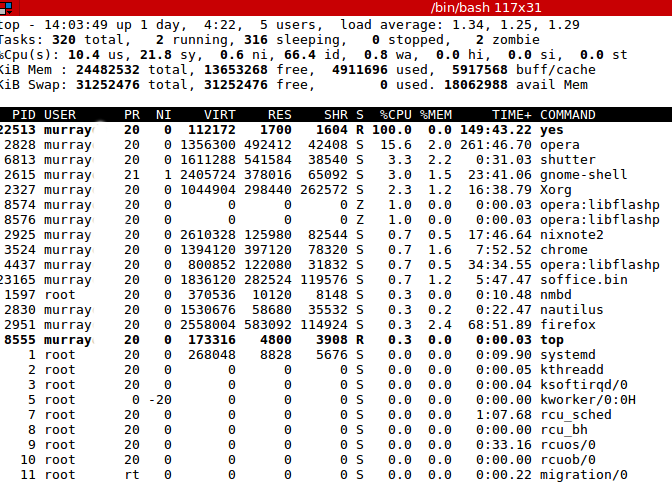
\includegraphics[scale=0.5]{figures/top_white}\\

\subsubsection{top's interactive commands}

\begin{tabularx}{\linewidth}{>{\bfseries}X | X} % the X is needed to wrap text
\caption{top's interactive commands}\label{table:top-controls}\\ % title of Table
\toprule
\normalfont{Command} & Action \\% inserts table heading, unbolds 1st column heading
\midrule
h & display help for interactive commands\\[2mm]	
d or s & set update interval \\[2mm]
x & highlight current sort field, display metrics in bold\\[2mm]
u & change effective user to monitor or all users\\[2mm]
l or t or m & toggles to hide/display\emph{ top's} top line (load), next two lines (tasks and \% cpu), last two lines (memory and swap info)\\[2mm]	
k & kill a task by PID\\[2mm]
r & renice a task by PID\\[2mm]	
f and s and enter & set sort field\\[2mm]
f and space & toggles display\\[2mm]
f and right-arrow to select and up/down arrow to move & moving field column\\[2mm]
q & quit top window and return to command prompt\\[2mm]
\bottomrule
\end{tabularx}

\subsubsection{top at the command line}

We can start a \keyword{top} session from the command line passing various parameters and settings to the \emph{top}.

\begin{table}[!h]
\caption{Using \emph{top} at the command line}
\begin{tabular}{|>{\bfseries}l p{12cm}|}
\hline
\normalfont{Command} & Action \\\hline
top -n1 -b | head -10 & Run only one iteration of the \keyword{top} command. This prints 10 lines which results in only the top 3 processes listed due to 5 lines for the Summary Area, a blank line, the table heading, and then the task area. So, only 3 lines left for the process list. If you use this method, add \# of processes you want to 7 for the \emph{head} option. This issue is addressed in the next command.\\[3mm]
top -b -d5 -n10 -u mgc & Run 10 iterations of \emph{top} with a 5 second delay for processes belonging to user \emph{mgc}. All processes are listed for \emph{mgc}, 10 distinct \emph{top} tables are generated. Each table displays the 5 lines of the Summary Area as well as all processes for user mgc.\\[3mm]
\multicolumn{2}{|l|}{\textbf{top -n1 | egrep -v "top|Tasks|Cpu|Mem|Swap"}}\\
& Run 1 iteration of the \emph{top} command, but remove the top 5 lines of the Summary Area, that is, the lines beginning with these keywords.\\[3mm]	
\multicolumn{2}{|l|}{\textbf{top | egrep -v "top|Tasks|Cpu|Mem|Swap|PID" | tee -a top.log}}\\
& Run and display the \emph{top} command until you manually end the command...and \emph{tee} the output to the file \textsl{top.log}, remove the top five lines of the Summary Area and the table headings for the task area.\\[3mm]
\hline
\end{tabular}
\end{table}

\subsection{hop over to htop}

\textit{I recommend that you install the \keyword{htop} package}. This package is a more user-friendly version of \emph{top}. I will not display more than the initial \emph{htop} screen that appears after you type the \emph{htop} command. Like, \emph{top}, the \emph{htop} window is created using \emph{ncurses.} For more information, please see this \href{https://en.wikipedia.org/wiki/Ncurses}{ncurses} URL. \emph{htop} has a menu driven system at the bottom of the screen. However, some of the function keys will be captured by your operating system and even by your terminal window. It is best just to click the menus using your mouse. 

\begin{description}
	\item[htop's advantages over top]
\end{description}
\begin{itemize}
	\item \tbi{more intuitive:} You can quickly grasp how to interact with \emph{htop} whereas you would have to use \emph{top's} help menu.
	\item \tbi{enhanced interactive commands:} Interactive commands are more numerous and powerful.
	\item \tbi{scroll vertically and horizontally:} With \emph{top} information can be clipped. With \emph{htop}, you can scroll horizontally to reveal all the information.
	\item \tbi{mouse driven:} You can use the mouse to select items and then use the menu system or interactive commands.
	\item \tbi{tree view available:} You can see a processes hierarchy, that is, see the parent-child relationship.
	\item \tbi{killing and renicing:} These tasks can be done without entering PIDs. Instead use the mouse  to select and then the menus to select the operation.
\end{itemize}

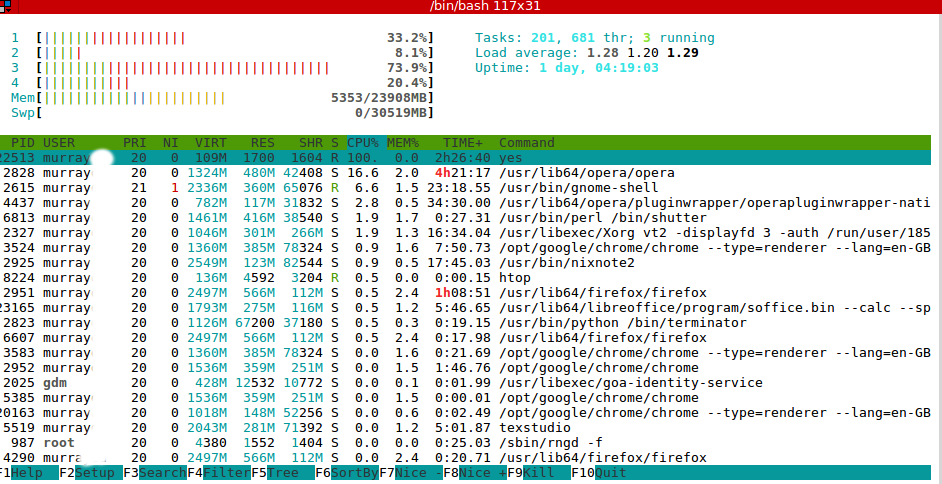
\includegraphics[scale=0.5]{figures/htop_white}\\

However, there is one area where \keyword{top} excels and exceeds the capability of \keyword{htop} and that is at the command line. Take a look at the number of options available to each command in the following section. I am using my \emph{.bashrc m-} function to show the options available to start each command.

Note, when \emph{top} is run in \emph{batch mode}, you cannot interact with \emph{top} as you can when \emph{top} is run in \emph{table mode}. That is, you cannot interrupt \emph{top} to issue the interactive commands.

\begin{lstlisting}[escapeinside={¿}{¿},frame=single,breaklines,columns=fixed]
¿\tld¿ m- htop
-d --delay=DELAY
-C --no-color --no-colour
-h --help
-p --pid=PID,PID...
-s --sort-key COLUMN
-u --user=USERNAME
-v --version

¿\tld¿ m- top
-h | -v	:Help/Version
-b  :Batch-mode operation 
-c  :Command-line/Program-name toggle
-d  :Delay-time interval as:  -d ss.t (secs.tenths)
-H  :Threads-mode operation
-i  :Idle-process toggle
-n  :Number-of-iterations limit as:  -n number
-o  :Override-sort-field as:  -o fieldname
-O  :Output-field-names
-p  :Monitor-PIDs mode as:  -pN1 -pN2 ...  or  -pN1,N2,N3 ...
-s  :Secure-mode operation
-S  :Cumulative-time toggle
-u | -U	:User-filter-mode as:  -u | -U number or name
-w  :Output-width-override as:  -w [ number ]
\end{lstlisting}

\subsection{over the top to atop}

Another interesting tool that can be used alongside \keyword{top} and \keyword{htop} is \keyword{atop}. One advantage that this package has is that it gives a historical summary of system and process activity since the last boot. For help with interactive commands, just type \emph{h}. The \emph{atop} table is split in two. The top of the table shows information on processes, cpu and memory usage, disk usage, and network usage. The bottom of the table shows the historical system and process activity since the last boot.

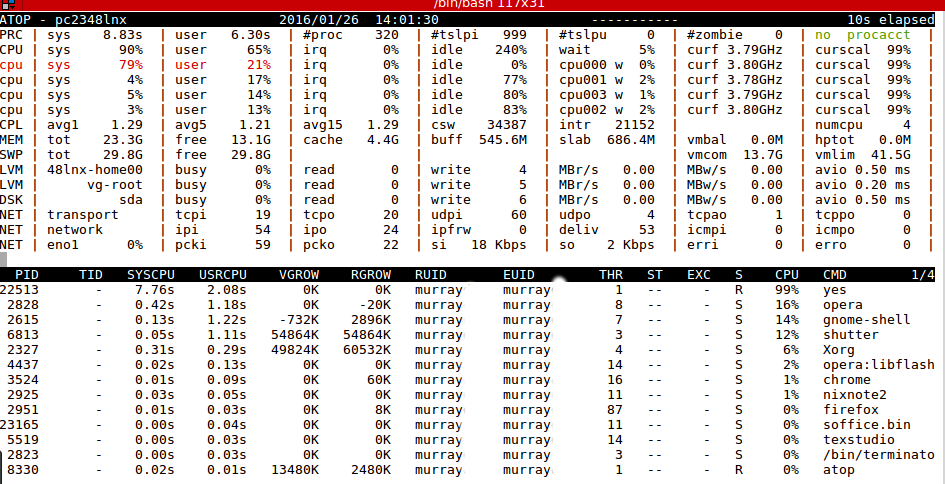
\includegraphics[scale=0.5]{figures/atop_white}

\textit{My suggestion is to use all three tools according to your needs.} 

\begin{description}
	\item[Summary of process monitoring tools as per manpages]
\end{description}
\begin{itemize}
	\item \tbi{top:} display Linux processes
	\item \tbi{htop:} interactive process viewer
	\item \tbi{atop:} Advanced System \& Process Monitor	
\end{itemize}

\section{killing processes}

\subsection{killall}

The following table lists some of the ways of killing or ending processes. \textit{Tread carefully...you are issuing these commands as \emph{sudo}}.

\begin{tabularx}{\linewidth}{>{\bfseries}X | X} % the X is needed to wrap text
\caption{killall}\label{table:killall}\\ % title of Table
\toprule
\normalfont{Command} & Action \\% inserts table heading, unbolds 1st column heading
\midrule
pgrep yes & list the process ids for all instances of the \emph{yes} command\\[2mm]
pgrep -u username yes & list process ids for \emph{yes} command for user \emph{username}\\[2mm]
killall yes & kill instances of \emph{yes} command...owned by you\\[2mm]
sudo killall yes & kill all instances of \emph{yes} command for all users...only root and sudoers can do this\\[2mm]
\bottomrule
\end{tabularx}

\begin{lstlisting}[escapeinside={¿}{¿},frame=single,breaklines,columns=fixed]
¿\tld¿ pgrep yes
6704
12307

¿\tld¿ pgrep -u mgc yes
12307

¿\tld¿ pgrep -u mgcr yes
6704
#
# I knew that both mgc and mgcr users had an instance of yes running. But suppose, you had a system with hundreds of users logged on. How would you get the yes PID for all users?
#
¿\tld¿ for users in `ps aux | awk '{ print $1 }' | sed '1 d' | sort | uniq`;do pgrep -u $users yes;done
12307
6704

¿\tld¿ killall yes
yes(12307): Operation not permitted
[1]+  Terminated              yes > /dev/null
#
# Note, the above command killed the mgcr instance of yes, but not the mgc instance. I issued the command as a non-root user mgcr. Only root and a user with sudo privileges such as the user mgcr can kill all instances.
#
¿\tld¿ sudo killall yes
#
# Has the mgc instance of yes been killed? Oh, yeah!
#
¿\tld¿ pgrep -u mgc yes
¿\tld¿ 
\end{lstlisting}

\subsection{finding all users running a process...a gotcha}\label{subsec:gotcha}

In the above section, I used a very interesting \emph{for} loop to get a list of all users running a process on my system. In order to find out who was logged on, I started by using the commands that are typically used to find who is logged on: \keyword{who}, \keyword{users}, and \keyword{finger}. However, these commands did not reveal all users. None of these commands revealed the user that had a current shell running off a bash shell. This is a \textbf{\color{red}serious} short coming of these commands! \\

\textbf{\color{red}Conclusion:} The commands \emph{who}, \emph{users}, and \emph{finger} do not list users that have bash shell sessions running at a different shell level!

\begin{lstlisting}[escapeinside={¿}{¿},frame=single,breaklines,columns=fixed]
#
# who -u or just who
#
¿\tld¿ who -u
mgcr tty2         2016-01-25 09:43  old         2321 (:0)
mgcr pts/0        2016-01-25 09:44 00:19        2823 (:0)
mgcr pts/1        2016-01-25 09:44   .          2823 (:0)
mgcr pts/2        2016-01-25 09:44 01:14        2823 (:0)
mgcr pts/3        2016-01-25 09:44 00:18        2823 (:0)
#
# Let's try the finger command...
#
¿\tld¿ finger
Login Name             Tty      Idle  Login Time   Office Office Phone Host
mgcr  Murray Davis   tty2       1d  Jan 25 09:43                     (:0)
mgcr  Murray Davis   pts/0      19  Jan 25 09:44                     (:0)
mgcr  Murray Davis   pts/1          Jan 25 09:44                     (:0)
mgcr  Murray Davis   pts/2    1:14  Jan 25 09:44                     (:0)
mgcr  Murray Davis   pts/3      18  Jan 25 09:44                     (:0)
#
# Let's try the users command...
#
¿\tld¿ users
mgcr mgcr mgcr mgcr mgcr
#
# But, just a second, I have another terminal window open for user mgcr and from this terminal I issued the 'su - mgc' command to switch to a bash session for this user. I then started the yes command from that bash window.
#
# From mgc's bash window, I issue these commands...
#
[mgc@LIB2015 ~]$ who -Hm
NAME     LINE         TIME             COMMENT
mgcr pts/3        2016-01-25 09:44 (:0)

[mgd@LIB2015 ~]$ echo $SHLVL
1
#
# Similarily, what's my shell level and psuedo terminal number for my mgcr terminal window?
#
¿\tld¿ who -Hm
NAME     LINE         TIME             COMMENT
mgcr pts/1        2016-01-25 09:44 (:0)

¿\tld¿ echo $SHLVL
2
#
# mgcr is running at shell level 2 and mgc is running at shell level 1
#
# Ok, let's get a unique list of all users running processes on my system using the ps command piped to other commands.
#
# | awk '{ print $1 }' - this first pipe gets only the first field of our output, the username
# | sed '1 d' - this second pipe says delete the first line of output, the heading, USER
# | sort  -  this third pipe says list the usernames in alphabetically order
# | uniq - the last pipe says, only show unique names
#
¿\tld¿ ps aux | awk '{ print $1 }' | sed '1 d' | sort | uniq
avahi
chrony
colord
dbus
gdm
mgc
mgcr
nobody
polkitd
root
rtkit
#
# Ok, assuming, yes is running for the mgc and mgcr users, let's filter the process list on yes.
#
¿\tld¿ ps aux | grep yes | awk '{ print $1 }' | sed '1 d' | sort | uniq
mgc
mgcr
#
# Now, let's use the who command. Notice that the who command  misses the mgc user who is logged into a bash shell window at a different shell level than mgcr.
#
¿\tld¿ who
mgcr tty2         2016-01-25 09:43 (:0)
mgcr pts/0        2016-01-25 09:44 (:0)
mgcr pts/1        2016-01-25 09:44 (:0)
mgcr pts/2        2016-01-25 09:44 (:0)
mgcr pts/3        2016-01-25 09:44 (:0)
\end{lstlisting}

\subsection{pkill and kill -9}

Ok, the following section shows how to kill user processes.


\begin{lstlisting}[escapeinside={¿}{¿},frame=single,breaklines,columns=fixed]
#
# We are logged on as 'mgcr'
#
¿\tld¿ whoami
mgcr
#
# First, let's get a list of all processes being run by user mgc, note that one of the processes is the actual bash window.
#
¿\tld¿ pgrep -l -u mgc
17628 bash
22962 yes
25761 sleep
#
# Alright, let's kill his sleep process.
#
¿\tld¿ pkill -u mgc sleep
pkill: killing pid 25761 failed: Operation not permitted
# 
# Oops, we have to be sudo, so let's use the abreviation for the previous command instead of retyping the command.
#
¿\tld¿ sudo !!
sudo pkill -u mgc sleep

¿\tld¿ pgrep -l -u mgc
17628 bash
22962 yes
#
# Ok, let's use a different method of killing another user's process.
# We are going to use command substitution indicated by the grave accents.
# We could have also used $(pgrep -u mgc yes).
#
¿\tld¿ sudo kill -9 `pgrep -u mgc yes`

¿\tld¿ pgrep -l -u mgc
17628 bash
#
# Alright, so mgc just has his bash session open, he has no other processes running.
#
# Meanwhile, back at mgc's command prompt, he issues the command 'who -Hm'. The output shows that mgcr is logged on. As well, we can see that the yes process was killed and the sleep process terminated. It is possible that it was mgcr who killed mgc's processes!
#
[mgc@LIB2015 ~]$ who -Hm
NAME LINE         TIME             COMMENT
mgcr pts/3        2016-01-25 09:44 (:0)
[1]-  Killed                  yes > /dev/null
[2]+  Terminated              sleep 1000

[mgc@LIB2015 ~]$ echo $SHLVL
1
#
# Let's switch back to the mgcr terminal and check what processes mgc is running. Notice that -bash appears beneath the CMD field, the - indicates that this process is a login shell.
#
¿\tld¿ ps -fu mgc
UID        PID  PPID  C STIME TTY          TIME CMD
mgc       6545  6528  0 13:45 pts/3    00:00:00 -bash
#
# Ok, let's kill the bash session belonging to mgc...which logs him off.
#
¿\tld¿ sudo pkill -u mgc bash
#
# Here is what we see at the mgc bash window.
#
[mgc@LIB2015 ~]$ logout
¿\tld¿ 
#
# Let's log back on as mgc and to see if we can find out who logged us off.
#
¿\tld¿ su -mgc

[mgc@LIB2015 ~]$ who -Hm
NAME  LINE        TIME             COMMENT
mgcr pts/3        2016-01-25 09:44 (:0)
#
# So, the answer is possibly...We can speculate because mgcr is the only user who is logged and who may have logged out mgc.
#
\end{lstlisting}

\subsection{ps and pgrep - more examples}

\begin{lstlisting}[escapeinside={¿}{¿},frame=single,breaklines,columns=fixed]
#
# List all bash sessions.
#
¿\tld¿ pgrep -d, -x bash
9619,9622,9629,9638
#
# Let's try different delimiters between the PIDs.
#
¿\tld¿ pgrep -d\; -x bash
9619;9622;9629;9638

¿\tld¿ pgrep -d\| -x bash
9619|9622|9629|9638
#
# Let's get detailed information on each bash session.
#
¿\tld¿ ps -fp `pgrep -x bash`
UID    PID  PPID  C STIME TTY      STAT   TIME CMD
mgcr  9619  9610  0 14:11 pts/0    SNs+   0:00 /bin/bash
mgcr  9622  9610  0 14:11 pts/1    SNs    0:00 /bin/bash
mgcr  9629  9610  0 14:11 pts/2    SNs+   0:00 /bin/bash
mgcr  9638  9610  0 14:11 pts/3    SNs+   0:00 /bin/bash
#
# Hey, that's interesting. I wonder what would happen if on psuedo terminal 3 (pts/3) we instead issued the command: 'su - mgc' and then repeated our command.
#
¿\tld¿ ps -fp `pgrep -x bash`
UID    PID  PPID  C STIME TTY      STAT   TIME CMD
mgcr  9619  9610  0 14:11 pts/0    SNs+   0:00 /bin/bash
mgcr  9622  9610  0 14:11 pts/1    SNs    0:00 /bin/bash
mgcr  9629  9610  0 14:11 pts/2    SNs+   0:00 /bin/bash
mgcr  9638  9610  0 14:11 pts/3    SNs    0:00 /bin/bash
mgc  11274 11260  0 14:23 pts/3    SN+    0:00 -bash
#
# Under the CMD column, for pts/3, two different pieces of information are shown. The original bash session for mgcr with PID 9638, the parent. The bash login session for mgc is listed next, the child.
#
# Light-bulb: At this point, a light bulb went on and I realised that there was another way to find all users that are logged on. Stay tuned for the explanation...or, click to go there ¿\hyperref[subsec:finduserprocs]{now}¿.
#
# Can we list the proces IDs for multiple users?
#
¿\tld¿ pgrep -u chrony,dbus
951
1008
#
# Let's try to get a little more infomration. It looks like PID 1008 belongs to chrony.
#
¿\tld¿ pgrep -lu chrony,dbus
951 dbus-daemon
1008 chronyd
#
# Ok, but let's be certain as to who owns the processes?
#
¿\tld¿ ps -fp `pgrep -u chrony,dbus`
UID        PID  PPID  C STIME TTY      STAT   TIME CMD
dbus       951     1  0 Jan25 ?        Ssl    0:02 /usr/bin/dbus-daemon --system --address=systemd: --nofork --nopidf
chrony    1008     1  0 Jan25 ?        S      0:00 /usr/sbin/chronyd
#
# Task: Find all processes for all users except: nobody.  We first need to get a list of all users present on the system.
#
¿\tld¿ ps aux | awk '{print $1}' | sed '1 d' | sort | uniq
avahi
chrony
colord
dbus
gdm
lp
mgc
mgcr
nobody
polkitd
root
rtkit

# Ok, let's use pgrep's inverse or -v option.
# Note, this is not a practical way of listing the processes for nobody. I am just using this example to illustrate one use of the inverse switch. You would instead issue this command: 'pgrep -lu nobody'.
#
¿\tld¿ pgrep -lvu avahi,chrony,colord,dbus,gdm,lp,mgd,mgcr,polkitd,root,rtkit
1862 dnsmasq
#
# Let's get the details...note, we have to remove the -l switch.
#
¿\tld¿ ps -fp `pgrep -vu avahi,chrony,colord,dbus,gdm,lp,mgd,mgcr,polkitd,root,rtkit`
UID        PID  PPID  C STIME TTY          TIME CMD
nobody    1862     1  0 Jan25 ?        00:00:00 /sbin/dnsmasq --conf-file=/var/lib/libvirt/dnsmasq/default.conf --lea

\end{lstlisting}

\subsubsection{finding all users running a process...revisited}\label{subsec:finduserprocs}

In the previous section, \hyperref[subsec:gotcha]{finding all users running a process...a gotcha}, I said that the light bulb went on. Here continues my adventure...

\begin{lstlisting}[escapeinside={¿}{¿},frame=single,breaklines,columns=fixed]
#
# The light-bulb went on while I was working on the previous section.
# We can use the following command to find users who are logged onto a 'bash login session' and as well 'bash terminal sessions'. Let's first find all 'bash sessions'.
#
¿\tld¿ ps -fp `pgrep -x bash`
UID    PID  PPID  C STIME TTY      STAT   TIME CMD
mgcr  9619  9610  0 14:11 pts/0    SNs    0:00 /bin/bash
mgcr  9622  9610  0 14:11 pts/1    SNs    0:00 /bin/bash
mgcr  9629  9610  0 14:11 pts/2    SNs+   0:00 /bin/bash
mgcr  9638  9610  0 14:11 pts/3    SNs    0:00 /bin/bash
mgc      11274 11260  0 14:23 pts/3    SN+    0:00 -bash
#
# Ugh, that's unwieldly! But, we know that if we want just 'bash login sessions', we just have to look for -bash under the CMD column.
#
# Here is the only way that I could get just that line, using command substitution.
#
¿\tld¿ ps -fp `pgrep -x bash` | awk '$9 == "-bash" {print}'
mgc      11274 11260  0 14:23 pts/3    SN+    0:00 -bash

# So, mgc is logged onto a 'bash login session' on pts/3. I next logged this user onto pts/0 and changed his shell from bash to sh and logged back out. Note that the command prompt changed from ¿\tld¿ to sh-4.3$ when I changed my shell.
#
¿\tld¿ su - mgc
Password: 

¿\tld¿$ chsh -s /bin/sh
Changing shell for mgc.
Password: 
Shell changed.
sh-4.3$ exit
#
# Note, I had to logout and back on to the pts/0 before I could list all 'sh login sessions' from another terminal window. On pts/0, I issue these commands.
#
¿\tld¿$ su - mgc
Password: 

sh-4.3$ echo $SHELL
/bin/sh
sh-4.3$ 
#
# Now, from my mgcr terminal window, I enter this command to get all sh shells. Note, there is no STAT column, there are only 8 columns, whereas when listing bash shells there were 9 columns. On pts/2, I issue these commands. If there are no current sh sessions, you will get an error if you issue the following command.  So, you would want to send errors to /dev/null.
#
¿\tld¿ ps -fp `pgrep -x sh`
UID        PID  PPID  C STIME TTY          TIME CMD
mgc     16780 16768  0 15:06 pts/0    00:00:00 -sh
#
# Since there are only 8 columns, we would have to awk on the 8th field .
#
¿\tld¿ ps -fp `pgrep -x sh` | awk '$8 == "-sh" {print}'
mgc      16780 16768  0 15:06 pts/0    00:00:00 -sh
#
# We would only have to use the longer command with the pipe to awk, if the default shell on the system was sh. We would only want the 'sh login sessions' indicated by -sh and not the regular 'sh terminal sessions' indicated by /bin/sh.
#
# Remember, if you wanted to be absolutely sure that you found all users regarless of the shell that they were using, you would have to look for all types of shells...which can be found with the chsh command. 
#
¿\tld¿ chsh --list-shells
/bin/sh
/bin/bash
/sbin/nologin
/usr/bin/sh
/usr/bin/bash
/usr/sbin/nologin
/usr/bin/tmux
/bin/tmux
/usr/bin/zsh
/bin/zsh
#
# You could create a command similar to the 'ps -fp' command for each type of shell. However, we need to address the error when there are no current sessions for the selected shell. I only show a part of the actual error message. When I issued this command, I had no current 'sh login sessions' open.
#
¿\tld¿ ps -fp `pgrep -x sh` | awk '$9 == "-sh" {print}'
error: list of process IDs must follow -p
#
# So, let's send the error message to the black hole. Note where I put the '2 > /dev/null' which is used to send stderr to the black hole. If you put this code section at the end of the command you would still get the error message.
# 
¿\tld¿ ps -fp `pgrep -x sh` 2 > /dev/null | awk '$9 == "-sh" {print}'
¿\tld¿
\end{lstlisting}

\subsection{sending commands to another terminal window}

This may appear as somewhat trivial, but suppose you wanted to send a command to another terminal window using its pseudo terminal number.

\begin{lstlisting}[escapeinside={¿}{¿},frame=single,breaklines,columns=fixed]
#
# How many terminal windows do I have open? I can simply list the files in the /dev/pts folder. ptmx is the psuedoterminal master/slave. I will not cover this concept. Below, we see that I have 4 pseudo terminal sessions open that are numbered 0 to 3.
#
# What is my pseudo terminal number?
#
¿\tld¿ who -Hm
NAME     LINE         TIME             COMMENT
mgcr pts/1        2016-01-27 14:38 (:0)
#
# We can also simply type...
#
¿\tld¿ tty
/dev/pts/1
#
# And, it is this full path format that I will use to send my commands to another terminal session. But, first, what are the pseudo terminal numbers that are currently open?
#
¿\tld¿ ls /dev/pts
0  1  2  3  ptmx
#
# From pts/1, I want to send the ls command to pts/3. That is, I want to send the file/directory list of my current directory to pts/3. I would do this by redirecting the ls command to pseudo terminal 3's full dev path.
#
¿\tld¿ ls > /dev/pts/3
#
# To indicate that I am at pts/3, I issue the tty command.
#
¿\tld¿ tty
/dev/pts/3
#
# And, after I issue the ls command on pts/1, the following file list starts to appear at the blank pts/3 command prompt. I elided most of the output since the file list is quite long.
#
¿\tld¿ anaconda    login.keyring.bu   rpmbuild
anaconda.old    ls.man             Runtastic
.
.
LaTeX           Public             zdesktop
latextut.rar    roder.sh
#
# However, there is a problem. I have to hit the enter key at pts/3 to return to its command prompt.
#
\end{lstlisting}

Click \href{http://www.humbug.in/2010/utility-to-send-commands-or-data-to-other-terminals-ttypts/}{Pritak Sinha} who has developed a C script called \tbi{ttyecho}. I will not display the code, but here is how you would send the \emph{ls} command from pts/1 to pts/3.

\begin{lstlisting}[escapeinside={¿}{¿},frame=single,breaklines,columns=fixed]
sudo ttyechno -n /dev/pts/3 ls	
\end{lstlisting}

The above command would send the output of the current directory of the source pseudo terminal to the destination pseudo terminal along with a carriage return. The script works flawlessly! Note, you must precede the command with \emph{sudo}. Where would you place this script? Does \emph{sudo} know about its path? Refer to chapter 2 and the discussion of \hyperref[sec:sudo]{sudo's PATH setting}.

\subsection{Let's be nice and all just get along!}

\subsubsection{Introduction}

All processes run with an assigned priority level. You can change this priority level using two commands: \keyword{nice} and \keyword{renice}. The Linux Kernel manages all processes in order to allocate CPU time according to a complex algorithm that establishes priority. Thankfully, this priority level can be changed when we want to assign more or less CPU resources to a process.\\

The process priority ranges from -20 to +19, the metric is called the \emph{nice} value. Think inversely when it comes to the metric, -20 represents the highest priority and +19 represents the lowest priority. Also, \emph{nice} values are only integer values.

\subsubsection{finding out how nice we really are}

\begin{lstlisting}[escapeinside={¿}{¿},frame=single,breaklines,columns=fixed]
#
# Ok, let's start our trusty sleep command.
#
¿\tld¿ sleep 1000 &
[1] 15587
#
# How can we see sleep's nice value. Let's try a couple of commands that we have already used.
#
¿\tld¿ ps -fp `pgrep -x sleep`
UID    PID  PPID  C STIME TTY      TIME     CMD
mgcr 15587 24107  0 08:47 pts/1    00:00:00 sleep 1000
#
# Hmm, no nice column. Remember, pgrep -x sleep, provides the PID of sleep, so we could just issue this command.
#
¿\tld¿ ps -fp 15587
UID    PID  PPID  C STIME TTY      TIME     CMD
mgcr 15587 24107  0 08:47 pts/1    00:00:00 sleep 1000
#
# Alright, how about grepping sleep from our 'ps aux' output.
#
¿\tld¿ ps aux | grep sleep
mgcr 15587  0.0  0.0 112176   712 pts/1    S    08:47   0:00 sleep 1000
mgcr 17661  0.0  0.0 116996  2240 pts/1    S+   09:02   0:00 grep --color=auto sleep
#
# Two things annoying about this output. We see the pipe to, grep sleep, process listed and there are no headings.
#
¿\tld¿ ps aux | head -1 ; ps aux | grep sleep | grep -v grep
USER   PID %CPU %MEM    VSZ   RSS TTY      STAT START   TIME COMMAND
mgcr 17238  0.0  0.0 112176   796 pts/1    S    08:58   0:00 sleep 1000
#
# Well, that got rid of 'grep sleep'. We can also use && instead of the semi-colon.
#
¿\tld¿ ps aux | head -1 && ps aux | grep sleep | grep -v grep
USER   PID %CPU %MEM    VSZ   RSS TTY      STAT START   TIME COMMAND
mgcr 17238  0.0  0.0 112176   796 pts/1    S    08:58   0:00 sleep 1000
#
# But, gosh darn, we still don't see the nice value.
#
¿\tld¿ ps -eo %U%p%n | grep sleep
¿\tld¿ 
#
# Hey, nothing was returned. Why?
#
¿\tld¿ ps -eo %U%p%n%c | grep sleep
mgcr 15587   0 sleep
#
# Oh yeah, if I am grepping sleep which is the command, I have to include the command column (%c). So, I see that 0 is the nice value, but I want the heading.
#
¿\tld¿ ps -eo %U%p%n%c | head -1 && ps -eo %U%p%n%c | grep sleep
USER   PID  NI COMMAND
mgcr 15587   0 sleep
#
# Another way to see the nice value...
#
¿\tld¿ ps -al | head -1 && ps -al | grep sleep
F S   UID   PID  PPID  C PRI  NI ADDR SZ WCHAN  TTY          TIME CMD
0 S 1858215107 15587 24107  0 80 0 - 28044 hrtime pts/1  00:00:00 sleep
#
# Hmm, that did not line up... we can see that the 8th field is the nice value, which equals 0. Because of alignment issues it looks like the nice value is 80.  Let's first just get just the 8th column.
#
¿\tld¿ ps -al | head -1 | tr -s ' ' | cut -d ' ' -f 8 && ps -al | grep sleep | tr -s ' ' | cut -d ' ' -f 8
NI
0
#
# Yeah, and I am going to remember that command!
# tr -s ' ' convert any contiguous spaces to  a single space
# cut -d ' ' -f 8 use a space as a delimiter and get the 8th field
# the first command up to the && gets the heading
# the command after the && gets the actual 'nice' value for 'sleep'.
#
# There has to be an easier way! Also, I had to start a new sleep session since my previous one ended, hence the new PID.
#
¿\tld¿ ps -fl -C yes
F S UID    PID  PPID  C PRI  NI ADDR SZ WCHAN  STIME TTY          TIME CMD
0 R mgcr 19912 24107 99  93   0 - 28043 -      10:24 pts/1    00:18:28 yes
#
# And, we can also use this command...remember spaces in the list of field options leads to an error!
#
¿\tld¿ ps -o pid,user,nice -C sleep
PID   USER   NI
19912 mgcr   0
#
# Hey, how many seconds did I say to sleep?
#
¿\tld¿ ps h -o pid,user,nice,command -C sleep
PID   USER   NI COMMAND
19912 mgcr   0  sleep 10000
#
# I don't want the heading...I may be working on writing a script. This is counter intuitive, h means 'no heading'.
#
¿\tld¿ ps h -o pid,user,nice,command -C sleep
19912 mgcr   0 sleep 10000
#
# Ok, let's just get the nice value of sleep.
#
¿\tld¿ ps  h -o nice -C sleep
0
#
# Suppose we just know the PID of the command, not the command itself.
#
¿\tld¿ ps  h -o nice -p 19912
0
\end{lstlisting}

\subsubsection{nice to see you}
It turns out the the Kernel gives each new process a \emph{nice} value of 0. That is not the lowest \emph{nice} value, it is a mid-road value. Remember, \emph{nice} values range from -20 to +19.\\

\begin{itemize}
\item \tbi{\keyword{nice}} - use this command to set the \emph{nice} value for new commands
\item \tbi{\keyword{renice}} - use this command to modify the \emph{nice} value of existing commands
\item \tbi{\keyword{denice}} - \href{https://www.youtube.com/watch?v=JKYF_h2K7oU}{a  Key and Peel sketch on Youtube}
\end{itemize}

\begin{lstlisting}[escapeinside={¿}{¿},frame=single,breaklines,columns=fixed]
#
# We begin by killing our previous sleep session
#
¿\tld¿ killall sleep
[1]+  Terminated              sleep 100000
#
# Let's create a new sleep process with a nice value of 10...low priority, note we used -10, not 10. Confusing?
#
¿\tld¿ nice -10 sleep 1000 &
[1] 24361
#
# Let's just get the nice value of sleep.
#
¿\tld¿ ps  h -o nice -C sleep
10
#
# What if we wanted a nice value of -10 for our sleep command? That is, we wanted to give it a higher 'nice' value. To make it even more confusing, we have to preceed -10 with another minus sign...and we have to do this as root. This likely makes sense to those with a math background.
#
¿\tld¿ killall sleep
[1]+  Terminated              nice -10 sleep 1000
#
# Ok, let's try setting the nice value of sleep below zero.
#
¿\tld¿ nice --10 sleep 1000 &
[1] 26304
nice: cannot set niceness: Permission denied
#
# We could not set the nice value to -10, but the command to start sleep was successful. We just ended up with a sleep process with the default nice value of zero.
#
¿\tld¿ ps  h -o nice -C sleep
0
#
# We must be root to set a negative nice value. As explained above, we specify a negative value by preceding the metric with another negative sign. We see that we now have a second sleep process with a priority of -10 and a PID of 26356.
#
¿\tld¿ sudo nice --10 sleep 1001 &
[2] 26356
¿\tld¿ ps  h -o nice -C sleep
0
-10
#
# Let's 'killall' the sleep processes.
#
¿\tld¿ killall sleep
sleep(26360): Operation not permitted
[1]-  Terminated              nice --10 sleep 1000
#
# Obviously, a non-root user cannot kill a root process, but we did kill our sleep process.
#
¿\tld¿ sudo killall sleep
[2]+  Done                    sudo env PATH=$PATH nice --10 sleep 1001
#
# Hey, cool! 'sudo env PATH=$PATH' precedes our actual command. Remember that we created an 'alias sudo' in our .bashrc file. The reason that it appears now is that I began working on this section after I added that alias to my .bashrc.
#
\end{lstlisting}	

\textbf{Conclusion: }Only \emph{root} can create a process with a \keyword{nice} value below 0, i.e., high priority nice values. Let's now look at \keyword{renice}.\\

\subsubsection{Nice? I want to be nicer?}

\begin{lstlisting}[escapeinside={¿}{¿},frame=single,breaklines,columns=fixed]
# 
# Let's begin by killing any sleep session...hmm, sleep slept.
#
¿\tld¿ sudo killall sleep
sleep: no process found
#
# Instead of worrying about under sleeping, let's switch to our yes command.
#
¿\tld¿ yes > /dev/null &
[1] 28091
#
# Let's get a full listing of the yes process by command name.
#
¿\tld¿ ps -fl -C yes
F S UID    PID  PPID  C PRI  NI ADDR SZ WCHAN  STIME TTY          TIME CMD
0 R mgcr 28091  3079 99  80   0 - 28043 -      13:20 pts/0    00:00:13 yes
#
# Let's get a full listing of the yes process using its PID.
#
¿\tld¿ ps -fl -p 28091
F S UID    PID  PPID  C PRI  NI ADDR SZ WCHAN  STIME TTY          TIME CMD
0 R mgcr 28091  3079 99  80   0 - 28043 -      13:20 pts/0    00:00:25 yes
#
# Let's just get the nice value of the yes command.
#
¿\tld¿ ps  h -o nice -C yes
0
#
# Nah, I also want the PID, command, and nice fields.
#
¿\tld¿ ps axo pid,comm,nice  | grep yes
27312 yes               0
#
# Hmm, I don't like all that extra space after yes.
#
¿\tld¿ ps axo pid,comm,nice  | grep yes | tr -s " "
27312 yes 0
#
# We can give yes a lower priority, that is, a positive nice value.
#
¿\tld¿ renice 13 -p 28091
28091 (process ID) old priority 0, new priority 13
#
# Let's confirm.
#
¿\tld¿ ps  h -o nice -C yes
13
#
# But, we cannot give it a higher priority...and with renice we can use a single minus sign.
#
¿\tld¿ renice -13 -p 28091
renice: failed to set priority for 28091 (process ID): Permission denied

¿\tld¿ ps  h -o nice -C yes
13
#
# So, we need sudo.
#
¿\tld¿ sudo renice -13 -p 28091
28091 (process ID) old priority 13, new priority -13

¿\tld¿ ps  h -o nice -C yes
-13
#
# Ok, we had to sudo to give it a higher priority, can we now lower that priority? Obama!
#
¿\tld¿ renice 13 -p 28091
28091 (process ID) old priority -13, new priority 13

¿\tld¿ ps  h -o nice -C yes
13
#
# Ok, but can we increase the priority keeping it above 0? Seems not. We can lower it, but not raise it after we lower it...unless we are sudo.
#
¿\tld¿ renice 5 -p 28091
renice: failed to set priority for 28091 (process ID): Permission denied
#
# Can we reset the priority for all processes for a single user?
#
¿\tld¿ su - mgc
Password:
#
# At this point, we just have our shell process running.
# 
¿\tld¿ ps -u mgc
PID   TTY          TIME CMD
29302 pts/3    00:00:00 sh
29358 pts/3    00:00:00 ps
#
# Let's create two more processes.
#
¿\tld¿ sleep 100000 &
[1] 29382

¿\tld¿ yes > /dev/null &
[2] 29418
#
# What are our nice values?
#
¿\tld¿ ps h -o nice
0
0
0
0
#
# Let's see a bit more information.
#
¿\tld¿ ps h -o user,nice,command
mgc        2 -sh
mgc        2 sleep 100000
mgc        2 yes
mgc        2 ps h -o user,nice,command
#
# We are logged on as mgc. For all of our processes, we can lower the 'nice' value to 2.
#
¿\tld¿ renice 2 -u mgc
1000 (user ID) old priority 0, new priority 2
#
# Even our sh shell has a lower priority.
#
¿\tld¿ps h -o user,nice,command
mgc        2 -sh
mgc        2 sleep 100000
mgc        2 yes
mgc        2 ps h -o user,nice,command	
#
# And, as we learned above, we cannot suddenly try to increase the priority of all processes, for example, try to set all processes to a nice value of 1.
#
¿\tld¿ renice 1 -u mgc
renice: failed to set priority for 1000 (user ID): Permission denied
\end{lstlisting}

\subsubsection{summary}

Note: With some of the \keyword{ps} headings, we can use abbreviations. For example, you can use \emph{comm} for \emph{command}. In the examples below, I am using a \emph{pid} value of 1010, a \emph{nice} value of 12 a \keyword{renice} value of -13, a group name of \emph{mygrp}, and a process called \emph{yes}. Non-root users can increase  the nice value (lower the priority) of one of their processes, but they cannot decrease the nice value (increase the priority) even after they have previously increased the nice value of this process. Non-root users can only set a positive nice value for their processes. The \emph{root} user can set, \emph{nice}, and reset, \emph{renice}, any value of any process for any user.

\begin{tabularx}{\linewidth}{>{\bfseries}X | X} % the X is needed to wrap text
\caption{nice and renice}\label{table:nicely}\\ % title of Table
\toprule
\normalfont{Command} & Action \\% inserts table heading, unbolds 1st column heading
\midrule
ps axo pid,command,nice | less & Get a tabular, formatted-with-heading listing of all processes and pipe to \emph{less} so that you can \emph{spacebar} through the listing.\\[2mm]
ps -fl -C yes & Get a tabular, formatted with heading listing of all processes  named \emph{yes}\\[2mm]
ps -o pid,user,nice,command -C yes & Get a tabular, formatted-with-heading listing of all processes named \emph{yes}, but only show \emph{pid}, \emph{user}, \emph{nice}, and \emph{command} fields.\\[2mm]
ps -o pid,user,nice,command -p 1010 & Get a tabular, formatted-with-heading listing of the process for PID (1010), but only show \emph{pid}, \emph{user}, \emph{nice} value, and \emph{command} fields.\\[2mm]
ps  h -o nice -C yes & Just display the numerical \emph{nice} value of  processes named \emph{yes}.\\[2mm]
ps  h -o nice -p 1010 & Just display the numerical \emph{nice} value for \emph{pid} number 1010.\\[2mm]
nice -12 yes & Non-root and root user, start \emph{yes} with a positive \emph{nice} value of 12. Non-root users can only set \emph{nice} to positive values.\\[2mm]
nice 12 yes & Same as above. With \emph{nice}, the value can be -12, 12, +12. End result, \emph{nice} value of positive 12.\\[2mm]
sudo nice -{}-{}12 yes & To set a negative nice value,-12, use two consecutive negative signs. Only \emph{root} can set a negative \emph{nice} value.\\[2mm]
renice 12 -p 1010 & If teh starting nice value is 0, both non-root and root users, can change the \emph{nice} value from 1 to 20 for \emph{pid} number 1010. Non-root user can only lower his processes \emph{nice} values so the starting \emph{renice} value for a non-root user would be 1. That is, he could change a 0 to a 1. This example, for a non-root user assumes existing \emph{nice} value is between 0 and 11.\\[2mm]
Alternatives & Note, we can also use the optional \emph{-n} = nice number option instead of just supplying the nice number, but this option must always go first.\\[2mm]
renice -n 12 -p 1010 & Same as \emph{renice 12 -p 1010}.\\[2mm]
renice -n +12 -p 1010 & Same as above.\\[2mm]
sudo renice -12 -p 1010 &  Only root can set a negative \emph{nice} value. In the case of \emph{renice}, -12 does equal -12. \\[2mm]
sudo renice -n -13 -g mygrp & Change priority of all processes owned by group \emph{mygrp}.\\[2mm]
sudo renice -13 \tgr{pgrep -u mgcr} & Change priority of all processes owned by user \emph{mgcr}.\\[2mm]
sudo renice -13 -u mgcr & An even easier way to do this.\\[2mm]
\bottomrule
\end{tabularx}

\section{I got a grip on you - \keyword{lsof} and \keyword{fuser}}

Sometimes, when you try to delete a file, you will get a vaguely-worded error message saying that you cannot delete the file because it is locked by some process. So, how do you find that locking process? At times, you may also be curious as to what users are running a specific process.

\begin{tabularx}{\linewidth}{>{\bfseries}X | X} % the X is needed to wrap text
\caption{lsof and fuser}\label{table:processes-lsof}\\ % title of Table
\toprule
\normalfont{Command} & Action \\% inserts table heading, unbolds 1st column heading
\midrule
lsof \$(which sshd) & What users are running the \emph{sshd} process? That is, who is connected to my system using the \emph{ssh} protocol?\\[2mm]
lsof -u root & What processes is the \emph{root} user running?\\[2mm]	
lsof -c sshd & What calls are being made by the \emph{sshd} command?\\[2mm]
fuser -v /home/mgcr & What processes are attached to my home directory. The \emph{-v} option provides a header.\\[2mm]
fuser -km /home/mgcr & Kill all those processes attached to my home directory.\\[2mm]
\bottomrule
\end{tabularx}

\section{Limit the number of user processes}

A multi-user server with shared resources can easily become overloaded. We therefore may want to limit the number of connections any one user can have. Alternatively, on a high-performance server, we may actually want to increase the limits. For RHEL, CentOS, and Fedora systems there are a couple of key places where you can find information on resource limits.

\subsection{Key configuration information and files}

\begin{lstlisting}[escapeinside={¿}{¿},frame=single,breaklines,columns=fixed]
¿\tld¿ cat /proc/1/limits
Limit                     Soft Limit           Hard Limit           Units     
Max cpu time              unlimited            unlimited            seconds   
Max file size             unlimited            unlimited            bytes     
Max data size             unlimited            unlimited            bytes     
Max stack size            8388608              unlimited            bytes     
Max core file size        0                    unlimited            bytes     
Max resident set          unlimited            unlimited            bytes     
Max processes             95550                95550                processes 
Max open files            65536                65536                files     
Max locked memory         65536                65536                bytes     
Max address space         unlimited            unlimited            bytes     
Max file locks            unlimited            unlimited            locks     
Max pending signals       95550                95550                signals   
Max msgqueue size         819200               819200               bytes     
Max nice priority         0                    0                    
Max realtime priority     0                    0                    
Max realtime timeout      unlimited            unlimited            us
#
# Here is another way to get that information. Be careful, pay attention to units of measure. In the table above the 'max locked memory' is in bytes, 65536. But, in the output below, its metric is in kbytes, 64. 65536/1024= 64, there are 1024 kilobytes per byte. -S=soft limits, -H=hard limits. See, the description of soft and hard limits below.
# 
¿\tld¿ ulimit -Sa
core file size          (blocks, -c) 0
data seg size           (kbytes, -d) unlimited
scheduling priority             (-e) 0
file size               (blocks, -f) unlimited
pending signals                 (-i) 95550
max locked memory       (kbytes, -l) 64
max memory size         (kbytes, -m) unlimited
open files                      (-n) 1024
pipe size            (512 bytes, -p) 8
POSIX message queues     (bytes, -q) 819200
real-time priority              (-r) 0
stack size              (kbytes, -s) 8192
cpu time               (seconds, -t) unlimited
max user processes              (-u) 95550
virtual memory          (kbytes, -v) unlimited
file locks                      (-x) unlimited

¿\tld¿ ulimit -Ha
core file size          (blocks, -c) unlimited
data seg size           (kbytes, -d) unlimited
scheduling priority             (-e) 0
file size               (blocks, -f) unlimited
pending signals                 (-i) 95550
max locked memory       (kbytes, -l) 64
max memory size         (kbytes, -m) unlimited
open files                      (-n) 4096
pipe size            (512 bytes, -p) 8
POSIX message queues     (bytes, -q) 819200
real-time priority              (-r) 0
stack size              (kbytes, -s) unlimited
cpu time               (seconds, -t) unlimited
max user processes              (-u) 95550
virtual memory          (kbytes, -v) unlimited
file locks                      (-x) unlimited
#
# Is that true for my general user account? What are my open file limits? It turns out that root also has these limits!
#
¿\tld¿ ulimit -Sn; ulimit -Hn
1024
4096
#
# Can we see the ulimit for another user? We can, if we have sudo privileges.
#
¿\tld¿ sudo su -c "ulimit -Hn" mgc
4096
#
# Note, if you tried to get this information for mgc when logged on as a non-root user, you would be prompted for mgc's password. And, if you foo-bared the password or didn't know it, you would get the error message below.
#
¿\tld¿ su - mgc -c "ulimit -Hn"
Password: 
su: Authentication failure
#
# Note, there is no specific man page for ulimit since it is a bash builtin command. I use my mbib function to get just that man page info. This output will help explain the difference between the soft and hard limits.
#
¿\tld¿ mbib ulimit umask
ulimit [-HSTabcdefilmnpqrstuvx [limit]]
Provides control over the resources available to the shell and to processes started by it, on systems that allow such control.  The -H and -S options specify that the hard or soft limit is set  for the  given  resource.   A hard  limit cannot be increased by a non-root user once it is set; a soft limit may be increased up to the value of the hard limit. If neither -H nor -S is  specified, both the soft and hard limits are set.  The value of limit can be a number in the unit specified for the resource or one of the special values hard, soft, or unlimited, which stand  for the  current hard limit,  the  current soft limit, and no limit, respectively.  If limit is omitted, the current value of the soft limit of the resource is printed, unless the -H option is given.  When  more than  one resource is specified, the  limit  name and unit are printed before the value. Other options are interpreted as follows:
-a     All current limits are reported
-b     The maximum socket buffer size
-c     The maximum size of core files created
-d     The maximum size of a process data segment
-e     The maximum scheduling priority ("nice")
-f     The maximum size of files written by the shell and its children
-i     The maximum number of pending signals
-l     The maximum size that may be locked into memory
-m     The maximum resident set size (many systems do not honor this limit)
-n     The maximum number of open file descriptors (most systems do not allow this value to be set)
-p     The pipe size in 512-byte blocks (this may not be set)
-q     The maximum number of bytes in POSIX message queues
-r     The maximum real-time scheduling priority
-s     The maximum stack size
-t     The maximum amount of cpu time in seconds
-u     The maximum number of processes available to a single user
-v     The maximum amount of virtual memory available to the shell and, on  some systems, to its children
-x     The maximum number of file locks
-T     The maximum number of threads

If  limit is given, and the -a option is not used, limit is the new value of the specified resource. If no option is given, then -f is assumed.  Values are in 1024-byte increments, except for -t, which is  in seconds; -p, which is in units of 512-byte blocks; and -T, -b, -n, and -u, which are unscaled values.  The return status is 0 unless an invalid option or argument is supplied, or an error occurs while setting a new limit.  In POSIX Mode 512-byte blocks are used for the `-c' and `-f' options.
#
# The /etc/security folder contains many folders and files that can be viewed and edited in order to make changes to kernel limits. One key file is limits.conf. Note, by default it contains only comments that help explain its useage.
#
¿\tld¿ ls -la  /etc/security
total 92
drwxr-xr-x.   7 root root  4096 Jan 25 08:45 .
drwxr-xr-x. 167 root root 12288 Feb 15 07:46 ..
-rw-r--r--.   1 root root  4620 Aug 12  2015 access.conf
-rw-r--r--.   1 root root    82 Aug 12  2015 chroot.conf
.
.
-rw-r--r--.   1 root root  3635 Aug 12  2015 group.conf
-rw-r--r--.   1 root root  2422 Aug 12  2015 limits.conf
drwxr-xr-x.   2 root root  4096 Nov 16 13:33 limits.d
.
.
-rw-r--r--.   1 root root   419 Aug 12  2015 sepermit.conf
-rw-r--r--.   1 root root  2179 Aug 12  2015 time.conf

¿\tld¿ cat /etc/security/limits.conf
¿\tbi{\#}¿ /etc/security/limits.conf
¿\tbi{\#}¿
¿\tbi{\#}¿This file sets the resource limits for the users logged in via PAM.
¿\tbi{\#}¿It does not affect resource limits of the system services.
¿\tbi{\#}¿
¿\tbi{\#}¿Also note that configuration files in /etc/security/limits.d directory,
¿\tbi{\#}¿which are read in alphabetical order, override the settings in this
¿\tbi{\#}¿file in case the domain is the same or more specific.
¿\tbi{\#}¿That means for example that setting a limit for wildcard domain here
¿\tbi{\#}¿can be overriden with a wildcard setting in a config file in the
¿\tbi{\#}¿subdirectory, but a user specific setting here can be overriden only
¿\tbi{\#}¿with a user specific setting in the subdirectory.
¿\tbi{\#}¿
¿\tbi{\#}¿Each line describes a limit for a user in the form:
¿\tbi{\#}¿
¿\tbi{\#}¿<domain>        <type>  <item>  <value>
¿\tbi{\#}¿
¿\tbi{\#}¿Where:
¿\tbi{\#}¿<domain> can be:
¿\tbi{\#}¿        - a user name
¿\tbi{\#}¿        - a group name, with @group syntax
¿\tbi{\#}¿        - the wildcard *, for default entry
¿\tbi{\#}¿        - the wildcard %, can be also used with %group syntax,
¿\tbi{\#}¿                 for maxlogin limit
¿\tbi{\#}¿
¿\tbi{\#}¿<type> can have the two values:
¿\tbi{\#}¿        - "soft" for enforcing the soft limits
¿\tbi{\#}¿        - "hard" for enforcing hard limits
¿\tbi{\#}¿
¿\tbi{\#}¿<item> can be one of the following:
¿\tbi{\#}¿        - core - limits the core file size (KB)
¿\tbi{\#}¿        - data - max data size (KB)
¿\tbi{\#}¿        - fsize - maximum filesize (KB)
¿\tbi{\#}¿        - memlock - max locked-in-memory address space (KB)
¿\tbi{\#}¿        - nofile - max number of open file descriptors
¿\tbi{\#}¿        - rss - max resident set size (KB)
¿\tbi{\#}¿        - stack - max stack size (KB)
¿\tbi{\#}¿        - cpu - max CPU time (MIN)
¿\tbi{\#}¿        - nproc - max number of processes
¿\tbi{\#}¿        - as - address space limit (KB)
¿\tbi{\#}¿        - maxlogins - max number of logins for this user
¿\tbi{\#}¿        - maxsyslogins - max number of logins on the system
¿\tbi{\#}¿        - priority - the priority to run user process with
¿\tbi{\#}¿        - locks - max number of file locks the user can hold
¿\tbi{\#}¿        - sigpending - max number of pending signals
¿\tbi{\#}¿        - msgqueue - max memory used by POSIX message queues (bytes)
¿\tbi{\#}¿        - nice - max nice priority allowed to raise to values: [-20, 19]
¿\tbi{\#}¿        - rtprio - max realtime priority
¿\tbi{\#}¿
¿\tbi{\#}¿<domain>      <type>  <item>         <value>
¿\tbi{\#}¿
¿\tbi{\#}¿*               soft    core            0
¿\tbi{\#}¿*               hard    rss             10000
¿\tbi{\#}¿@student        hard    nproc           20
¿\tbi{\#}¿@faculty        soft    nproc           20
¿\tbi{\#}¿@faculty        hard    nproc           50
¿\tbi{\#}¿ftp             hard    nproc           0
¿\tbi{\#}¿@student        -       maxlogins       4
¿\tbi{\#}¿ End of file

\end{lstlisting}

\subsection{Temporary and permanent changes - examples}

Alright, now that we know where to find information on the kernel limits, let's start making some changes. Obviously, since you are messing around with kernel limits, you need to be \emph{root} in order to make the changes. Permanent changes are made by editing \textsl{/etc/security/limits.conf}. Temporary changes are made by using the \keyword{ulimit} command.

\begin{enumerate}
	\item{Bob - Bob is a pain in the ass. He runs an application that opens hundreds of files. Since the file size is unlimited, this tends to use up lots of resources. Let's edit \textsl{/etc/security/limits.conf} and add these lines:\\
		\textbf{bob soft nofile 100}\\
		\textbf{bob hard nofile 100}\\
		Now, instead of the maximum of 1024 files, Bob can only open 100 files.}
	\item{Executives - Members of the executive group watch streaming videos all day. These video files are enormous. Let's limit the file size for the executive group to 1GB or 1000000KB.\\
		\textbf{@executive hard data 1000000}}
	\item{Shackle everyone - Our main server is slowing down to a crawl. Let's temporary limit the number of user processes until we find out what's going on. We issue this command at the command line.\\
		\textbf{sudo ulimit -u 10000}}
\end{enumerate}




